\documentclass[10pt]{beamer}
\usetheme[
%%% option passed to the outer theme
%    progressstyle=fixedCircCnt,   % fixedCircCnt, movingCircCnt (moving is deault)
  ]{Berlin}
  
% If you want to change the colors of the various elements in the theme, edit and uncomment the following lines

% Change the bar colors:
%\setbeamercolor{Feather}{fg=red!20,bg=red}

% Change the color of the structural elements:
%\setbeamercolor{structure}{fg=red}

% Change the frame title text color:
%\setbeamercolor{frametitle}{fg=blue}

% Change the normal text color background:
%\setbeamercolor{normal text}{fg=black,bg=gray!10}

%-------------------------------------------------------
% INCLUDE PACKAGES
%-------------------------------------------------------

\usepackage[utf8]{inputenc}
\usepackage[english]{babel}
\usepackage[T1]{fontenc}
\usepackage{amsmath}
\usepackage{helvet}
\usepackage{multirow}
\usepackage{graphicx}
\usepackage{comment}
\usepackage[absolute,overlay]{textpos}
\usepackage{tabularx}
\usepackage{tikz}
\usetikzlibrary{arrows,automata,positioning}
\usetikzlibrary{shapes.multipart}
\usetikzlibrary{decorations.markings}
\usetikzlibrary{matrix}
\usepackage{marvosym}
\usepackage[marvosym]{tikzsymbols}

%-------------------------------------------------------
% DEFFINING AND REDEFINING COMMANDS
%-------------------------------------------------------

% colored hyperlinks
%\renewcommand*{\Footnotemark}[1]{\NCC@makefnmark{#1}}
\newcommand{\chref}[2]{
  \href{#1}{{\usebeamercolor[bg]{Feather}#2}}
}
\newcommand{\tuple}[1]{{\langle #1 \rangle}}
\newcommand{\pre}{\mathsf{pre}}     % precondition
\newcommand{\eff}{\mathsf{eff}}     % effect
\newcommand{\cond}{\mathsf{cond}}   % conditional effect

\newcommand{\X}{\mathcal{X}}
\newcommand{\F}{\mathcal{F}}
\newcommand{\A}{\mathcal{A}}
\newcommand{\N}{\mathcal{N}}
\newcommand{\I}{\mathcal{I}}
\newcommand{\real}{\mathbb{R}}
\newcommand{\Dw}{\mathcal{D}}
\newcommand{\Xw}{\mathcal{X}}
\newcommand{\Aw}{\mathcal{A}}
\newcommand{\Rw}{\mathcal{R}}
\newcommand{\OO}{\mathcal{O}}
\newcommand{\tOO}{\wt{\OO}}
\newcommand{\II}[1]{\mathbb{I}{\left\{#1\right\}}}
\newcommand{\PP}[1]{\mathbb{P}\left[#1\right]}
\newcommand{\EE}[1]{\mathbb{E}\left[#1\right]}
\newcommand{\EEs}[2]{\mathbb{E}_{#2}\left[#1\right]}
\newcommand{\PPt}[1]{\mathbb{P}_t\left[#1\right]}
\newcommand{\EEt}[1]{\mathbb{E}_t\left[#1\right]}
\newcommand{\PPi}[1]{\mathbb{P}_i\left[#1\right]}
\newcommand{\EEi}[1]{\mathbb{E}_i\left[#1\right]}
\newcommand{\EEp}[1]{\mathbb{E}_{\pi,P}\left[#1\right]}
\newcommand{\EEcp}[2]{\mathbb{E}_{\pi,P}\left[\left.#1\right|#2\right]}
\newcommand{\PPc}[2]{\mathbb{P}\left[#1\left|#2\right.\right]}
\newcommand{\PPct}[2]{\mathbb{P}_t\left[#1\left|#2\right.\right]}
\newcommand{\PPcc}[2]{\mathbb{P}\left[\left.#1\right|#2\right]}
\newcommand{\PPcct}[2]{\mathbb{P}_t\left[\left.#1\right|#2\right]}
\newcommand{\PPcci}[2]{\mathbb{P}_i\left[\left.#1\right|#2\right]}
\newcommand{\EEc}[2]{\mathbb{E}\left[#1\left|#2\right.\right]}
\newcommand{\EEcc}[2]{\mathbb{E}\left[\left.#1\right|#2\right]}
\newcommand{\EEcs}[3]{\mathbb{E}_{#3}\left[\left.#1\right|#2\right]}
\newcommand{\EEcct}[2]{\mathbb{E}_t\left[\left.#1\right|#2\right]}
\newcommand{\EEcci}[2]{\mathbb{E}_i\left[\left.#1\right|#2\right]}
\renewcommand{\th}{\ensuremath{^{\mathrm{th}}}}
\def\argmin{\mathop{\mbox{ arg\,min}}}
\def\argmax{\mathop{\mbox{ arg\,max}}}
\newcommand{\ra}{\rightarrow}

\newcommand{\norm}[1]{\left\|#1\right\|}
\newcommand{\onenorm}[1]{\norm{#1}_1}
\newcommand{\infnorm}[1]{\norm{#1}_\infty}
\newcommand{\iprod}[2]{\left\langle#1,#2\right\rangle}
\newcommand{\ev}[1]{\left\{#1\right\}}
\newcommand{\pa}[1]{\left(#1\right)}
\newcommand{\bpa}[1]{\bigl(#1\bigr)}
\newcommand{\Bpa}[1]{\Bigl(#1\Bigr)}
\newcommand{\sign}{\mbox{sign}}
\newcommand{\wh}{\widehat}
\newcommand{\wt}{\widetilde}
\newcommand{\transpose}{^\top}

\newcommand{\loss}{\ell}
\newcommand{\hloss}{\wh{\loss}}
\newcommand{\hL}{\wh{L}}
\newcommand{\tZ}{\wt{Z}}
\newcommand{\reg}{\mathfrak{R}}
\newcommand{\hreg}{\widehat{\reg}}
\newcommand{\hr}{\wh{r}}
\newcommand{\hv}{\wh{v}}
\newcommand{\hq}{\wh{q}}
\newcommand{\hmu}{\wh{\mu}}
\newcommand{\hR}{\wh{R}}
\newcommand{\tmu}{\wt{\mu}}
\newcommand{\tN}{\wt{N}}
\newcommand{\RE}[2]{\mbox{RE}\left(\left.#1\right\|#2\right)}
\newcommand{\KL}[2]{\mbox{KL}\left(#1\middle\lVert#2\right)}
\newcommand{\DD}[3]{D_{#3}\left(#1\middle\lVert#2\right)}
\newcommand{\DDC}[2]{\DD{#1}{#2}{C}}
\newcommand{\DDS}[2]{\DD{#1}{#2}{S}}

\newcommand{\trho}{\wt{\rho}}

\definecolor{gold}{rgb}{1,0.75,0}
\definecolor{darkred}{rgb}{0.75,0,0}
\setbeamercolor*{goldc}{fg=black,bg=gold}
\definecolor{darkpurp}{rgb}{0.4,0.2,0.4}
\setbeamercolor*{purpc}{fg=white,bg=darkpurp}
\setbeamercolor*{redc}{fg=white,bg=darkred}
\newcommand{\hG}[1]{\large \textcolor{darkred}{#1}}

\newcommand{\redd}[1]{\textcolor{darkred}{#1}}
\newcommand{\goldd}[1]{\textcolor{gold}{#1}}

\definecolor{ballblue}{rgb}{0.0, 0.5, 0.5}
\definecolor{lightgray}{rgb}{0.85, 0.85, 0.85}

%-------------------------------------------------------
% INFORMATION IN THE TITLE PAGE
%-------------------------------------------------------

\title[] % [] is optional - is placed on the bottom of the sidebar on every slide
{ % is placed on the title page
      \textbf{Machine Learning}
}

\author[Jonsson \& G\'omez]
{      Anders Jonsson \& \textbf{Vicen\c{c} G\'omez} \\
\vspace*{0.5cm}
Master in Intelligence Interactive Systems\\
2021-22\\
\vspace*{0.5cm}
Lecture 8\\
Deep Learning and Applications II
%      {\ttfamily bagchi.bhaskar@cse.iitkgp.ernet.in}
}

\date{}

\AtBeginSection[]
{
   \begin{frame}
       \frametitle{Content}
       \tableofcontents[currentsection]
   \end{frame}
}

%-------------------------------------------------------
% THE BODY OF THE PRESENTATION
%-------------------------------------------------------

\begin{document}

%-------------------------------------------------------
% THE TITLEPAGE
%-------------------------------------------------------

\begin{frame}[plain,noframenumbering] % the plain option removes the header from the title page, noframenumbering removes the numbering of this frame only
  \titlepage % call the title page information from above
\end{frame}

\begin{frame}
    \tableofcontents
\end{frame}

\section{Recap}


\begin{frame}
  \frametitle{History of deep learning}
  \begin{itemize}
	\item[1943] Computer model of artificial neuron [McCulloch and Pitts]
	\item[1960-70] Backpropagation algorithm for training neural networks [Kelley; Bryson; Dreyfus; Ivakhnenko; Lapa; Werbos]
	\item[1970-80] First AI winter
	\item[1980-86] Modern version of backpropagation [Linnainmaa; Fukushima; Parker; Rumelhart et al.]
	\item[1986-95] Second AI winter
	\item[1995-] Novel network models, faster processors, GPUs
	\item[2010-] Breakthrough of deep learning
  \end{itemize}
\end{frame}

\begin{frame}
\frametitle{Computational power}
%\centerline{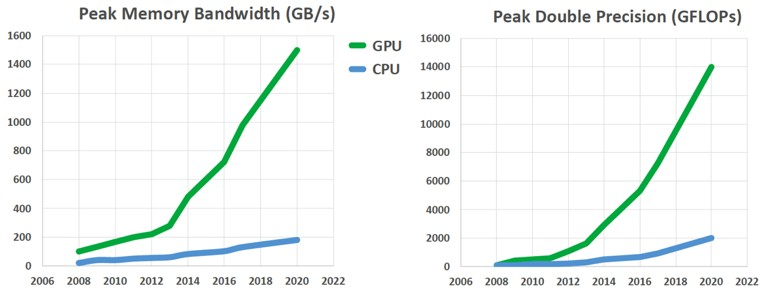
\includegraphics[height=5cm]{images/decade-gpu-natoli.jpg}}
\end{frame}


\section{Recurrent Neural Networks}

\begin{frame}
  \frametitle{Recurrent Neural Networks}
\begin{center}
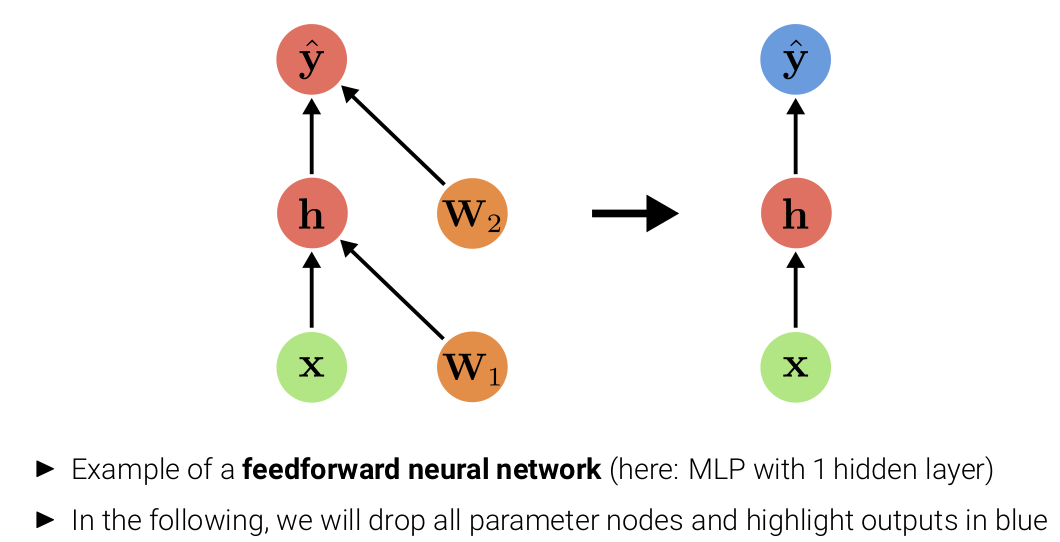
\includegraphics[width=.9\textwidth]{images/s1}
\end{center}
\end{frame}


\begin{frame}
  \frametitle{Feedforward vs Recurrent Neural Network}
\begin{center}
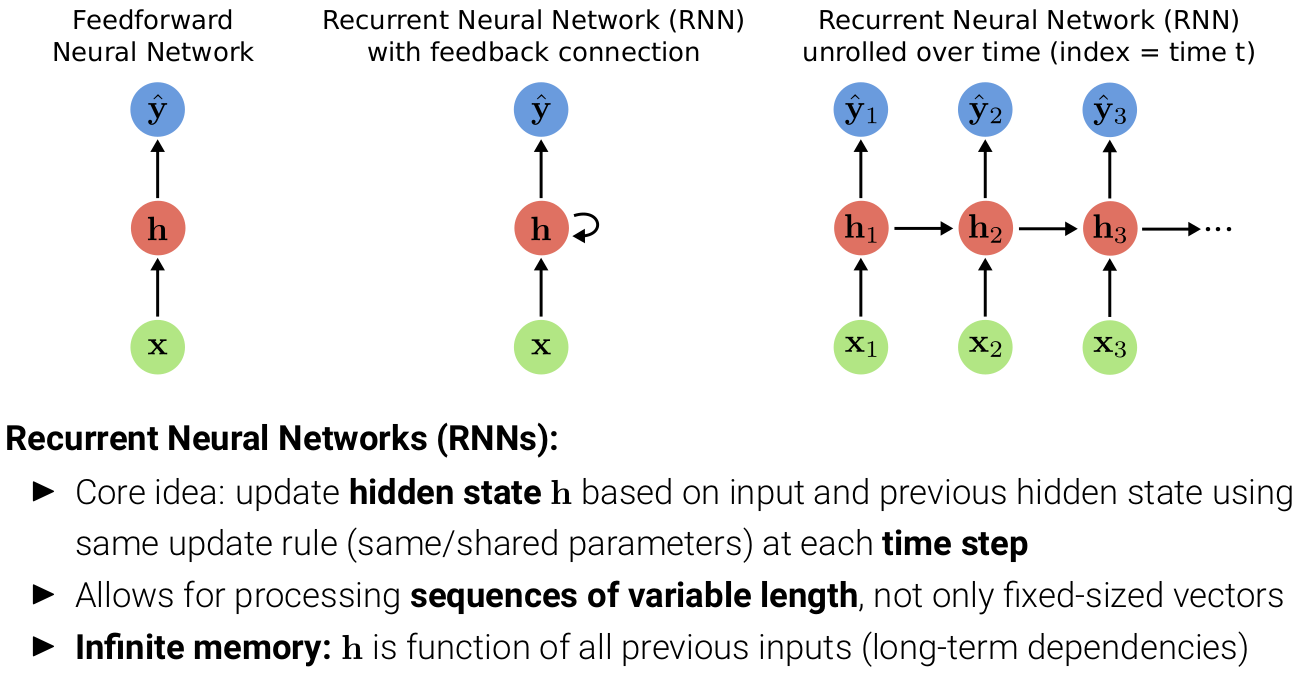
\includegraphics[width=.9\textwidth]{images/s2}
\end{center}
\end{frame}


\begin{frame}
  \frametitle{Basic Recurrent Neural Network}
\begin{center}
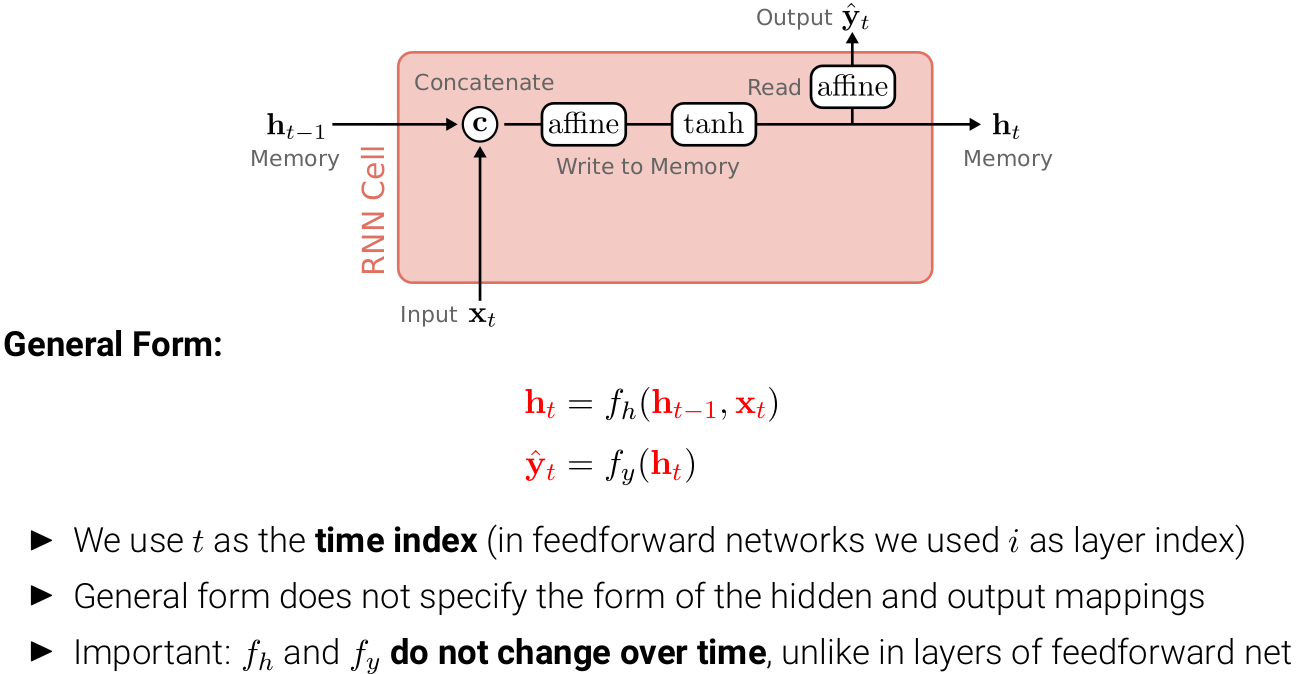
\includegraphics[width=.9\textwidth]{images/s3}
\end{center}
\end{frame}


\begin{frame}
  \frametitle{Basic Recurrent Neural Network}
\begin{center}
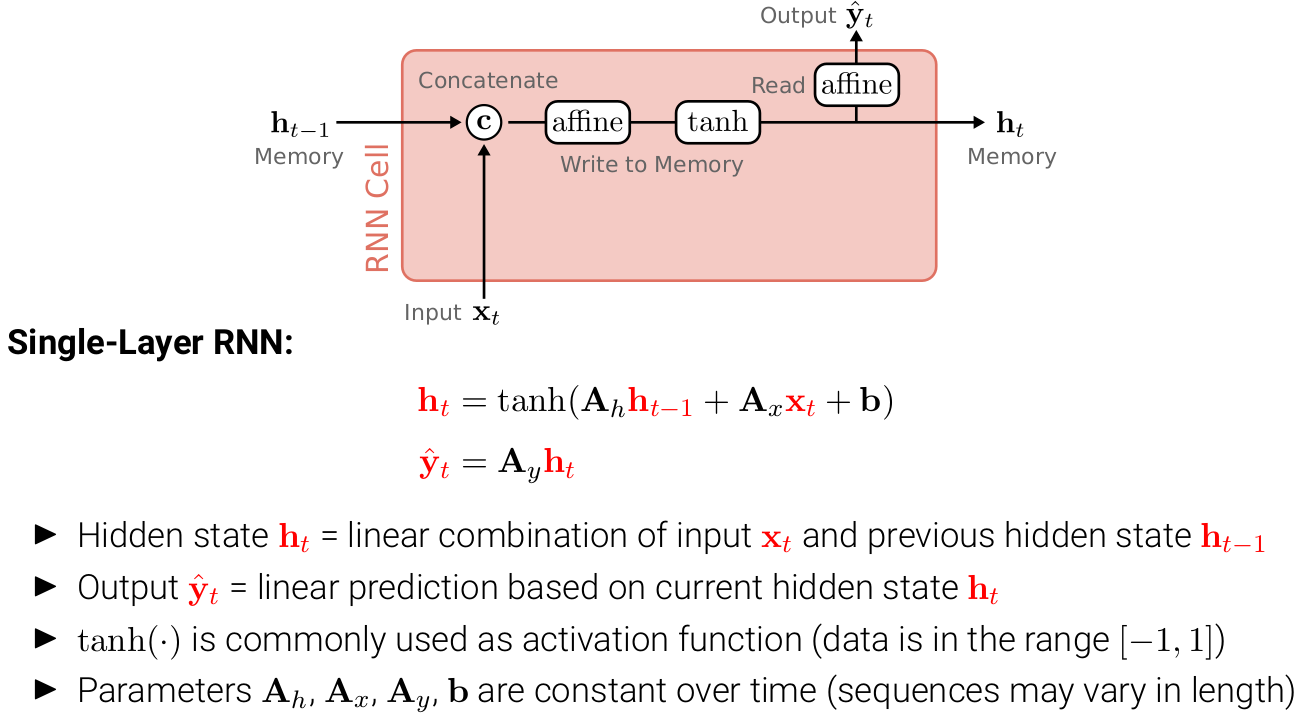
\includegraphics[width=.9\textwidth]{images/s4}
\end{center}
\end{frame}


\begin{frame}
  \frametitle{Mapping Types}
\begin{center}
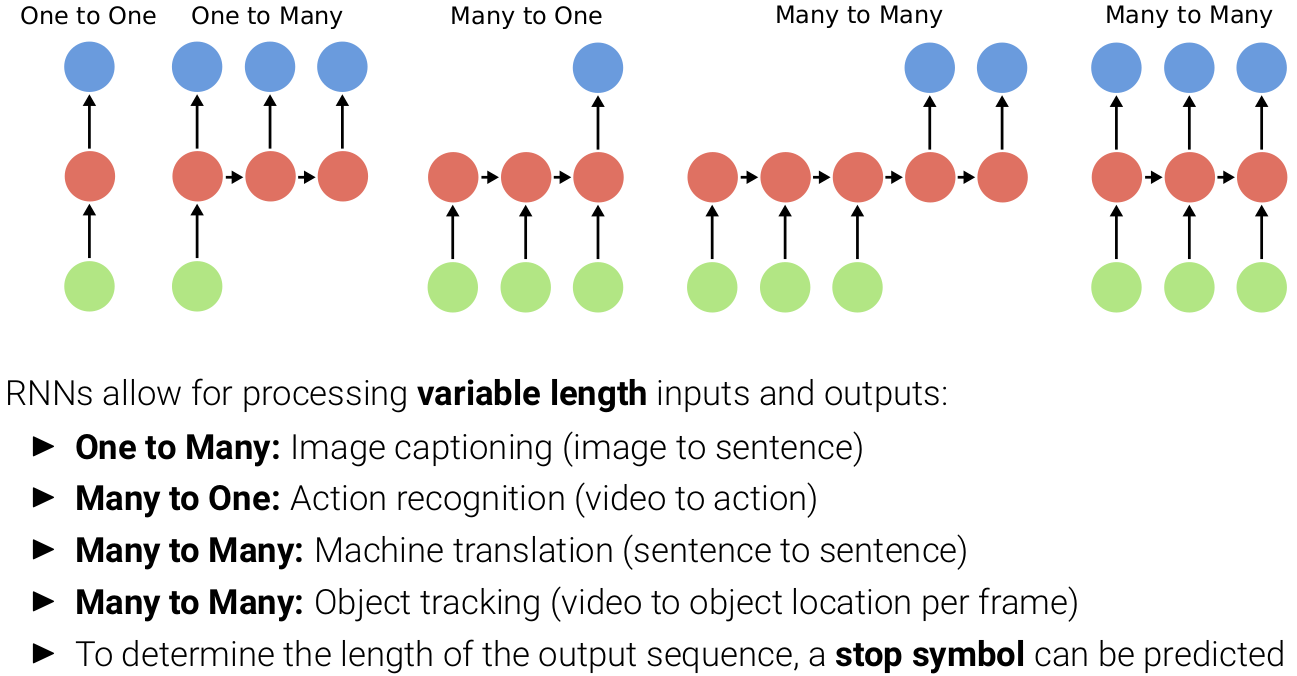
\includegraphics[width=.9\textwidth]{images/s5}
\end{center}
\end{frame}


\begin{frame}
  \frametitle{Backpropagation Through Time}
\begin{center}
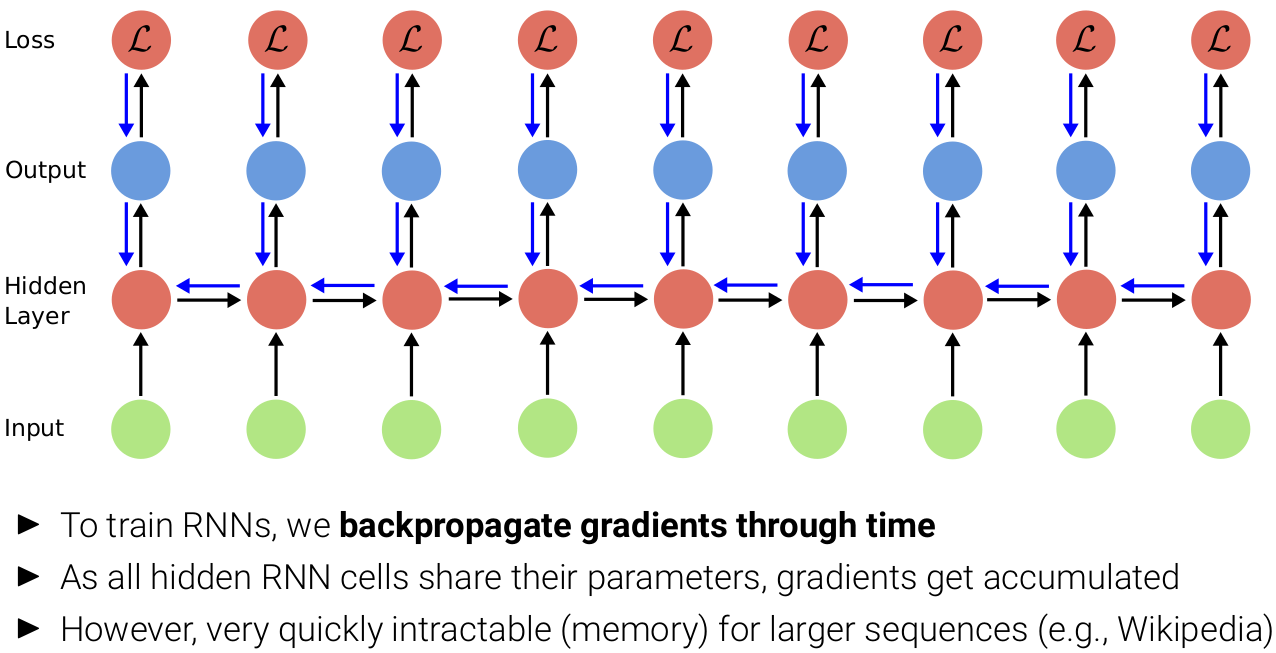
\includegraphics[width=.9\textwidth]{images/s6}
\end{center}
\end{frame}

\begin{frame}
  \frametitle{(Truncated) Backpropagation Through Time}
\begin{center}
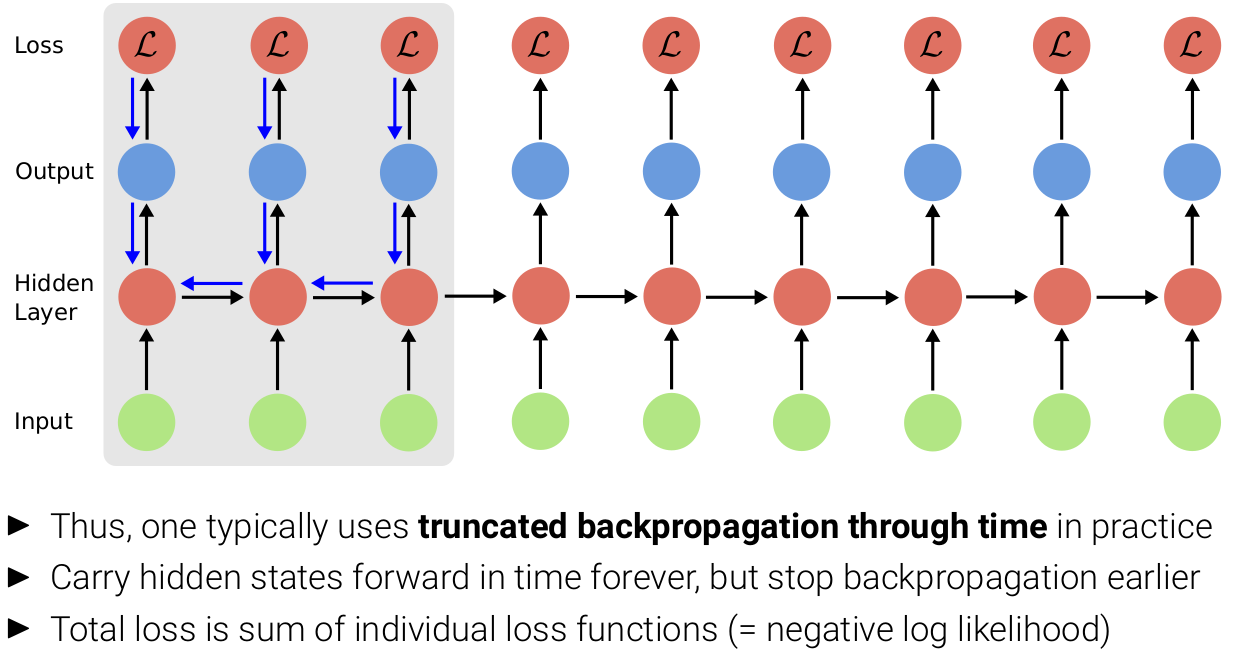
\includegraphics[width=.9\textwidth]{images/s7}
\end{center}
\end{frame}


\begin{frame}
  \frametitle{(Truncated) Backpropagation Through Time}
\begin{center}
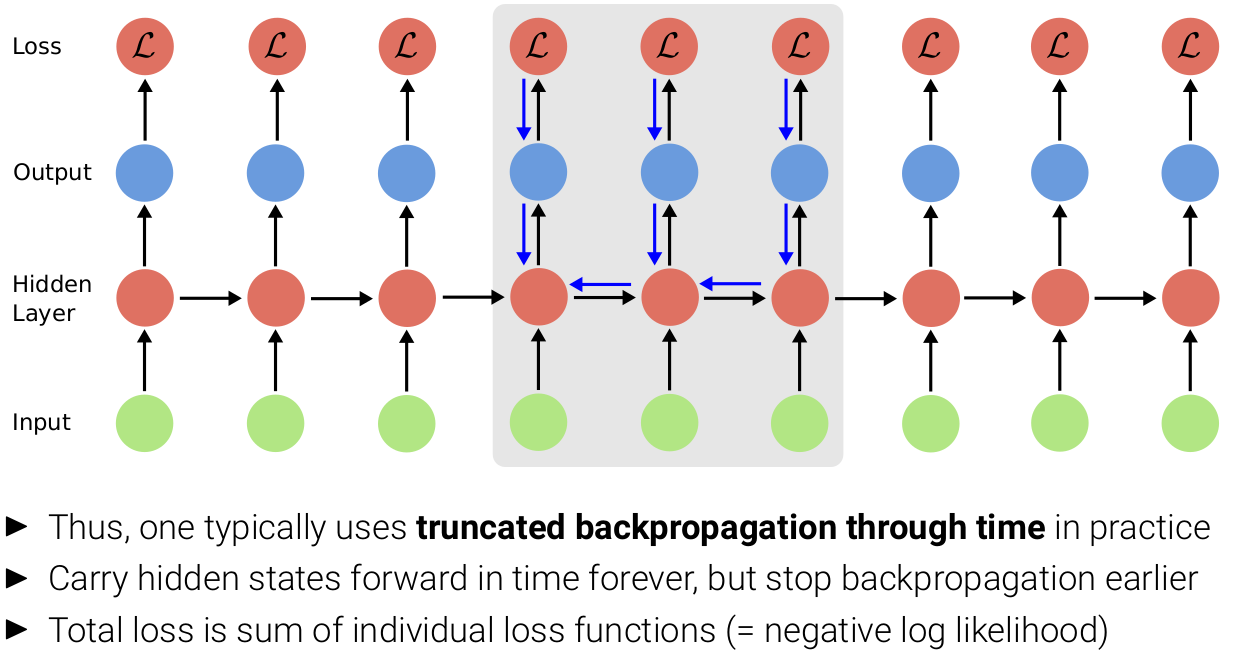
\includegraphics[width=.9\textwidth]{images/s8}
\end{center}
\end{frame}


\begin{frame}
  \frametitle{(Truncated) Backpropagation Through Time}
\begin{center}
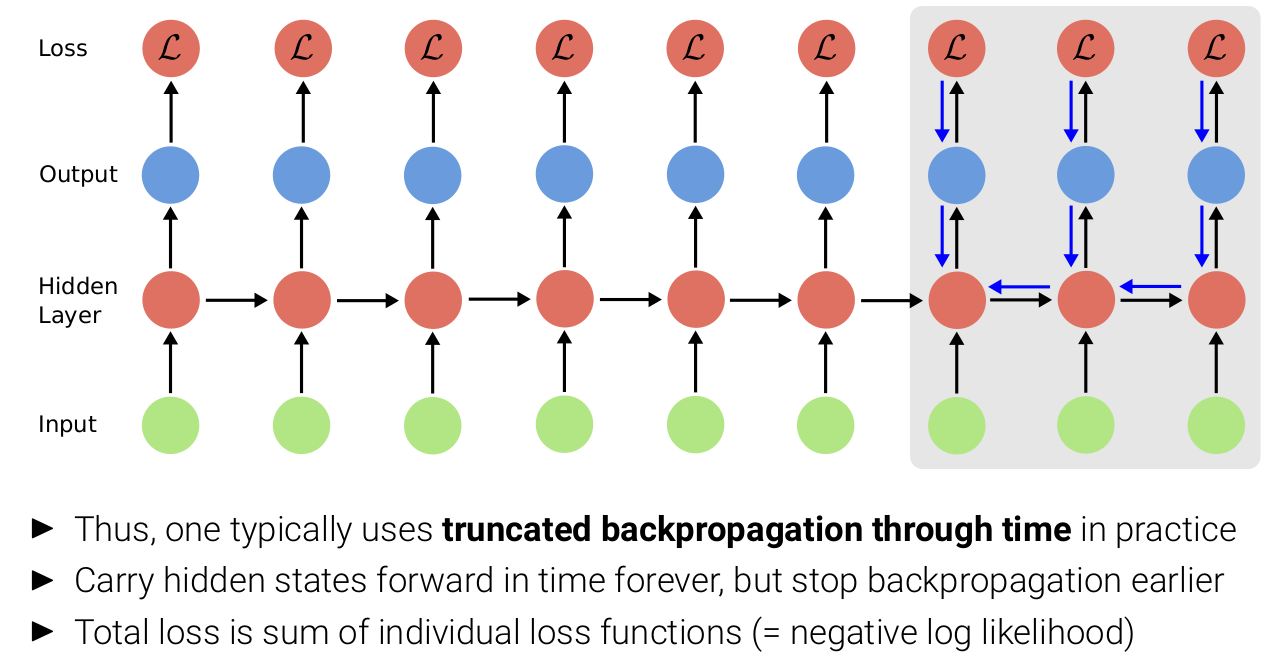
\includegraphics[width=.9\textwidth]{images/s9}
\end{center}
\end{frame}


\begin{frame}
  \frametitle{Multi-Layer RNNs}
\begin{center}
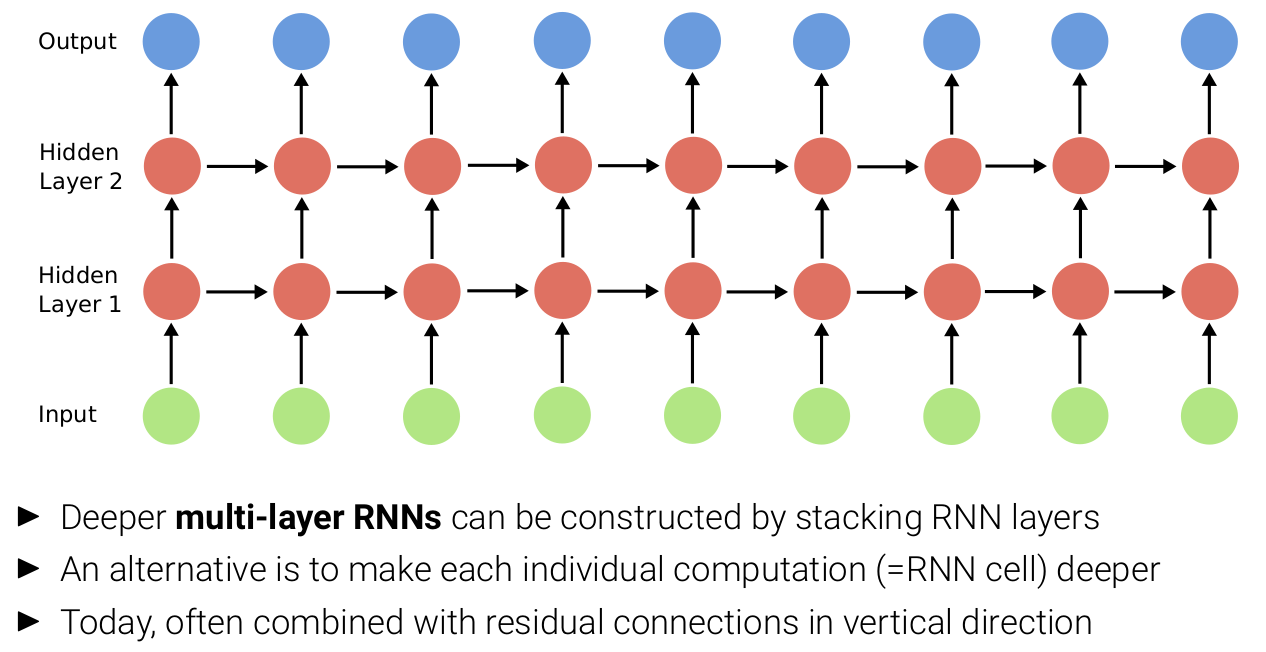
\includegraphics[width=.9\textwidth]{images/s10}
\end{center}
\end{frame}


\begin{frame}
  \frametitle{Limitations of Vanilla RNNs}
\textbf{What is the problem with vanilla RNNs?}
\begin{center}
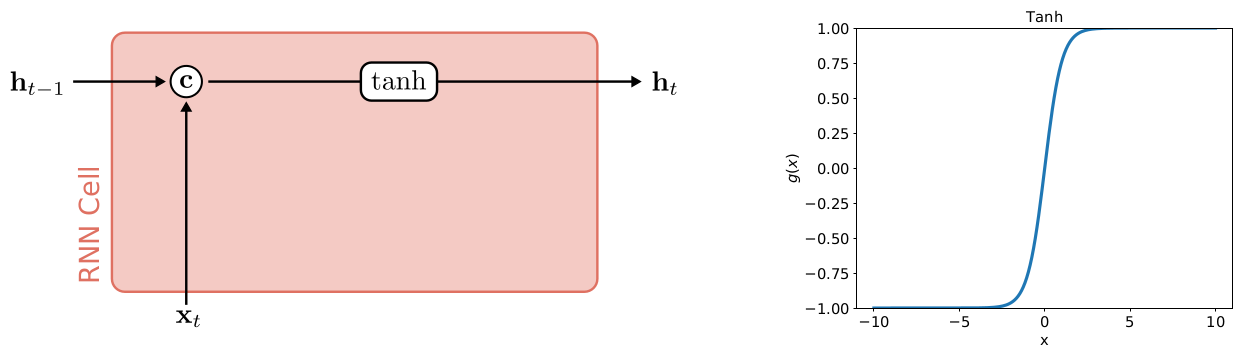
\includegraphics[width=.9\textwidth]{images/s11}
\end{center}
\vspace{-.25cm}
\begin{center}
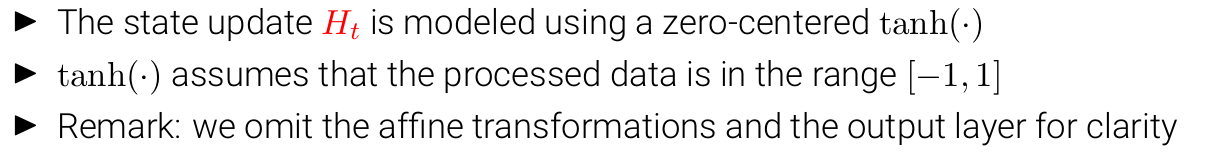
\includegraphics[width=.85\textwidth]{images/s12}
\end{center}
\end{frame}

\begin{frame}
  \frametitle{Vanishing-Exploding Gradients}
\begin{center}
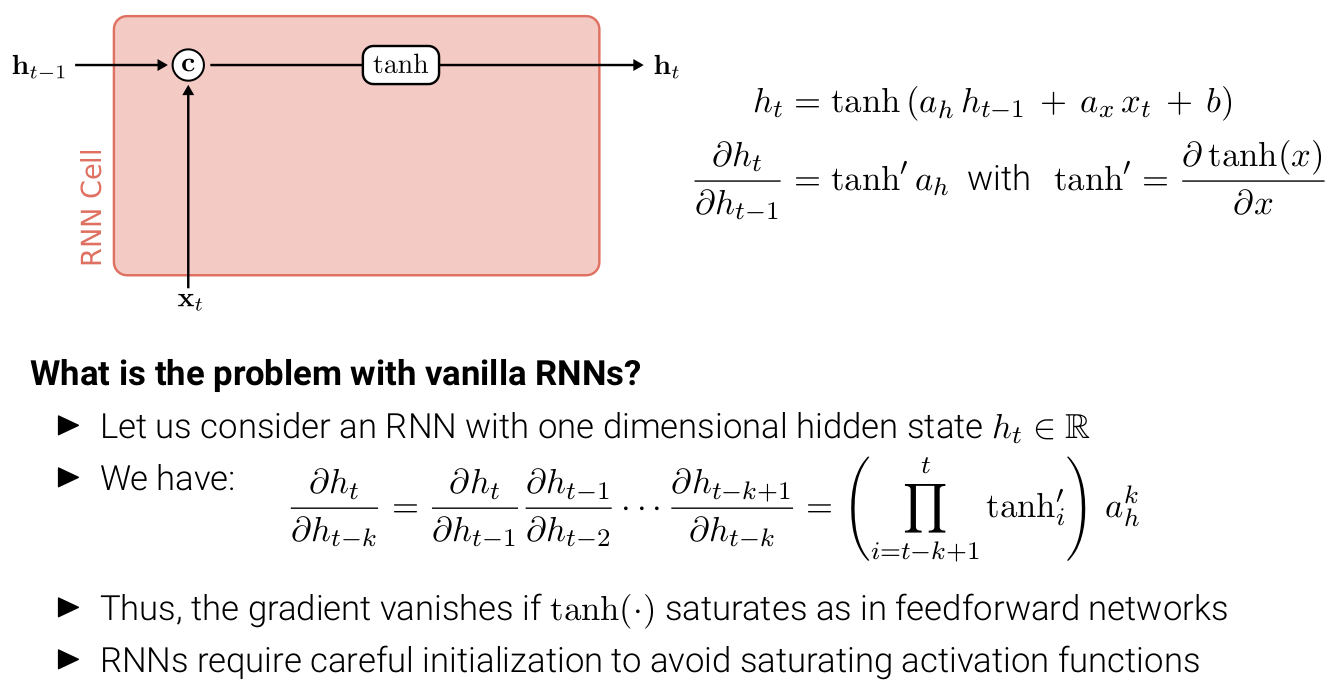
\includegraphics[width=.95\textwidth]{images/s13}
\end{center}
\end{frame}

\begin{frame}
  \frametitle{Vanishing-Exploding Gradients}
\begin{center}
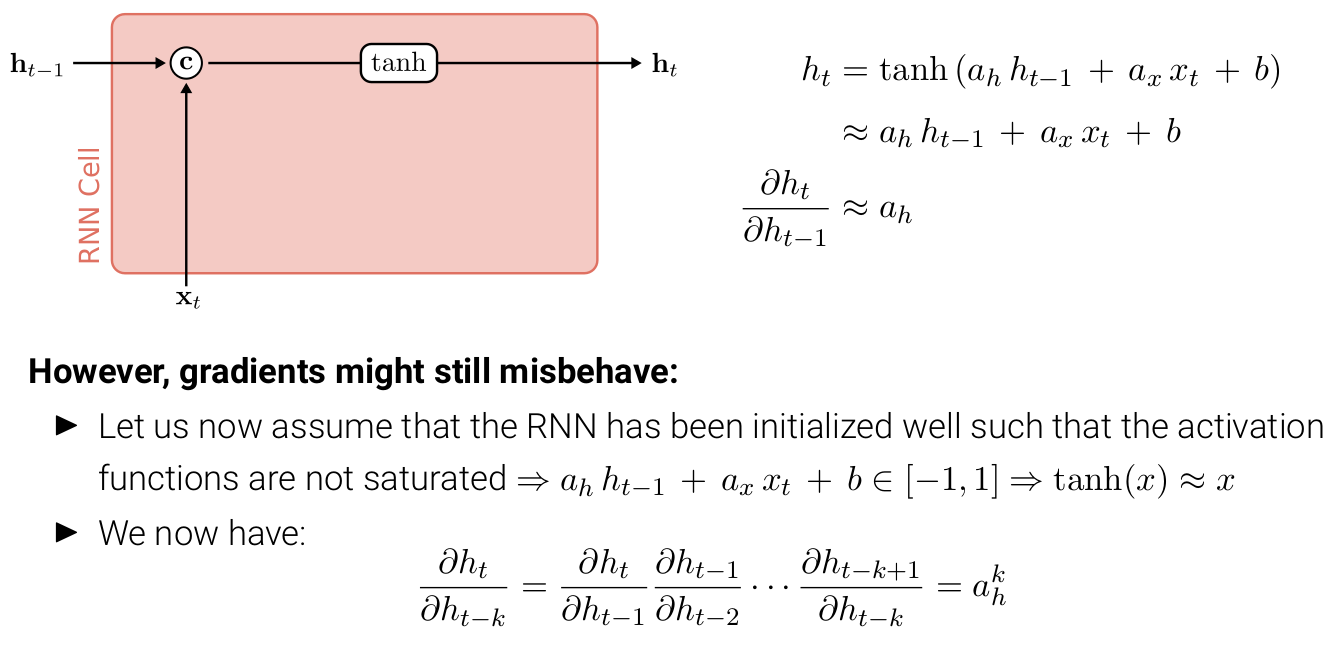
\includegraphics[width=.95\textwidth]{images/s14}
\end{center}
\end{frame}


\begin{frame}
  \frametitle{Vanishing-Exploding Gradients}
\begin{center}
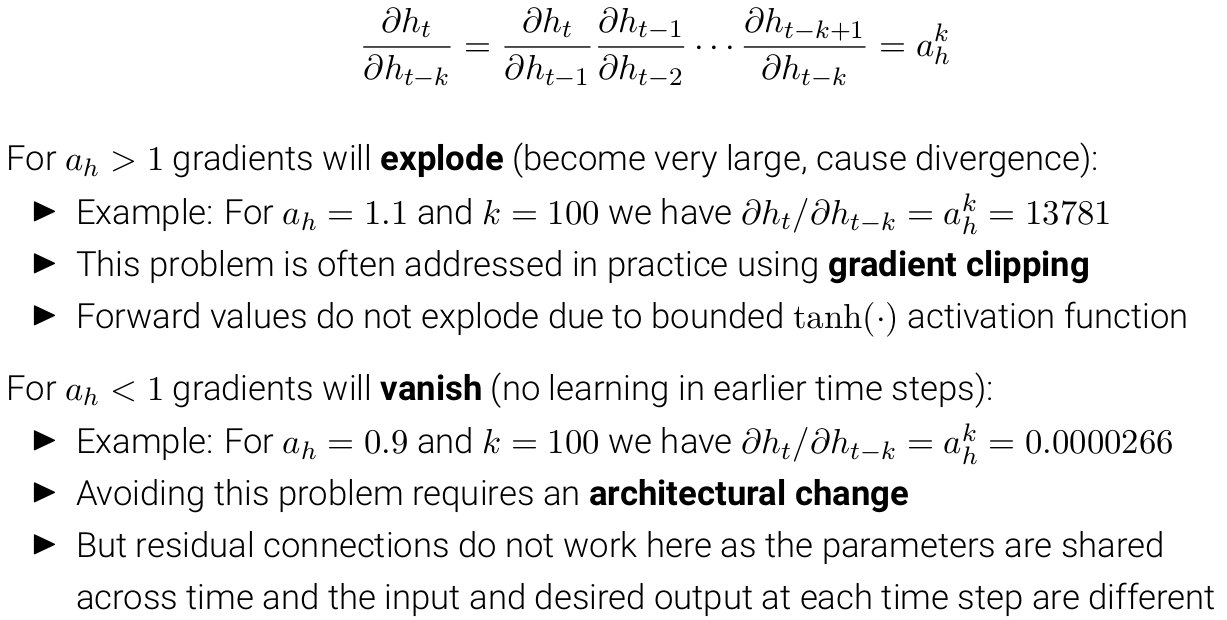
\includegraphics[width=.95\textwidth]{images/s15}
\end{center}
\end{frame}


\begin{frame}
  \frametitle{Gradient Clipping}
\begin{center}
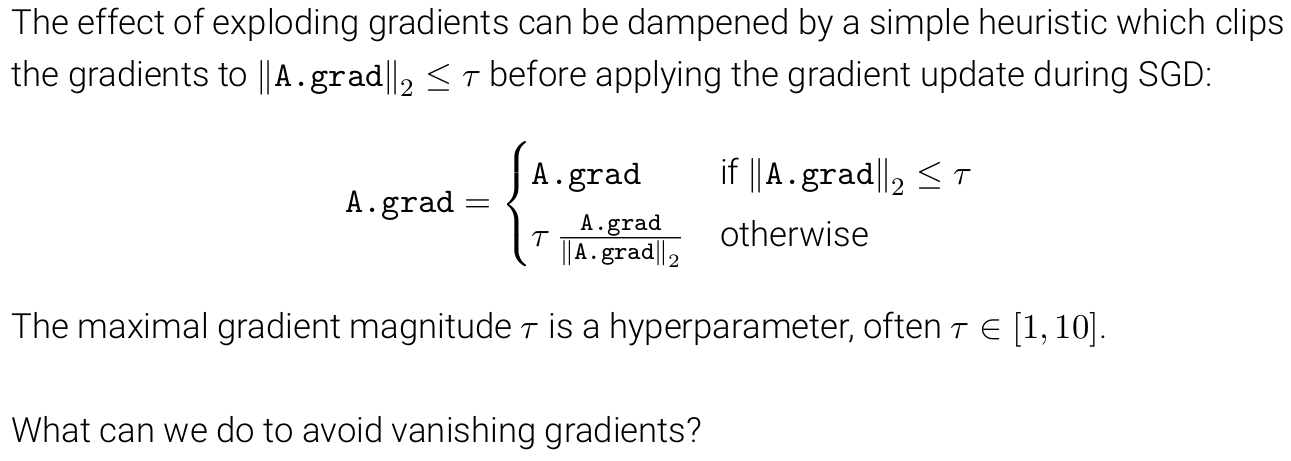
\includegraphics[width=.95\textwidth]{images/s16}
\end{center}
\end{frame}

\begin{frame}
  \frametitle{Gated Recurrent Networks}
\begin{center}
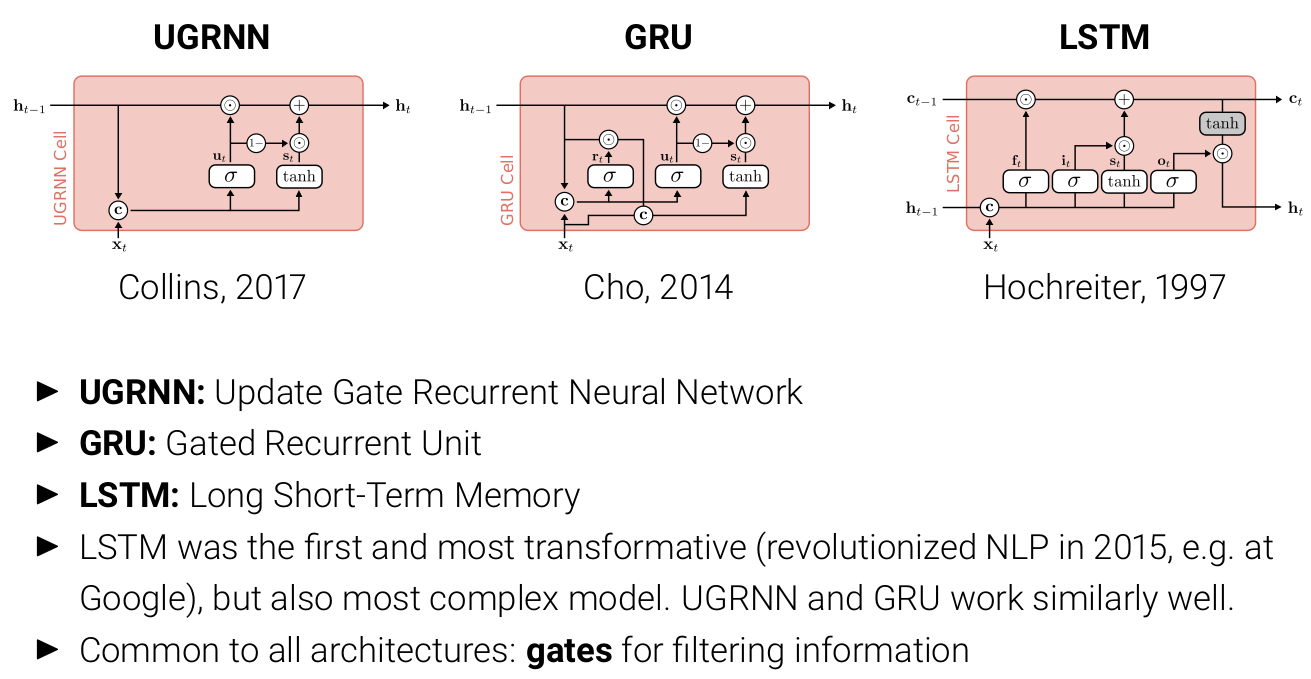
\includegraphics[width=.95\textwidth]{images/s17}
\end{center}
\end{frame}

\begin{frame}
  \frametitle{Gradient Flow}
\begin{center}
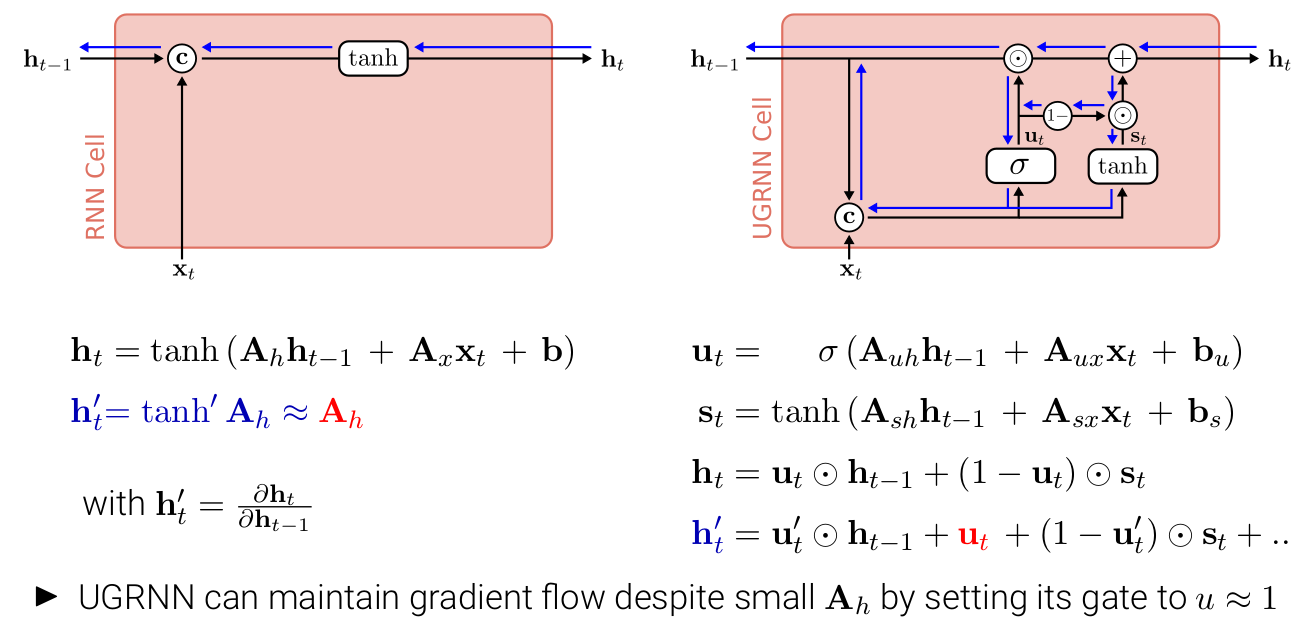
\includegraphics[width=.95\textwidth]{images/s18}
\end{center}
\end{frame}

\begin{frame}
  \frametitle{Gradient Flow}
\begin{center}
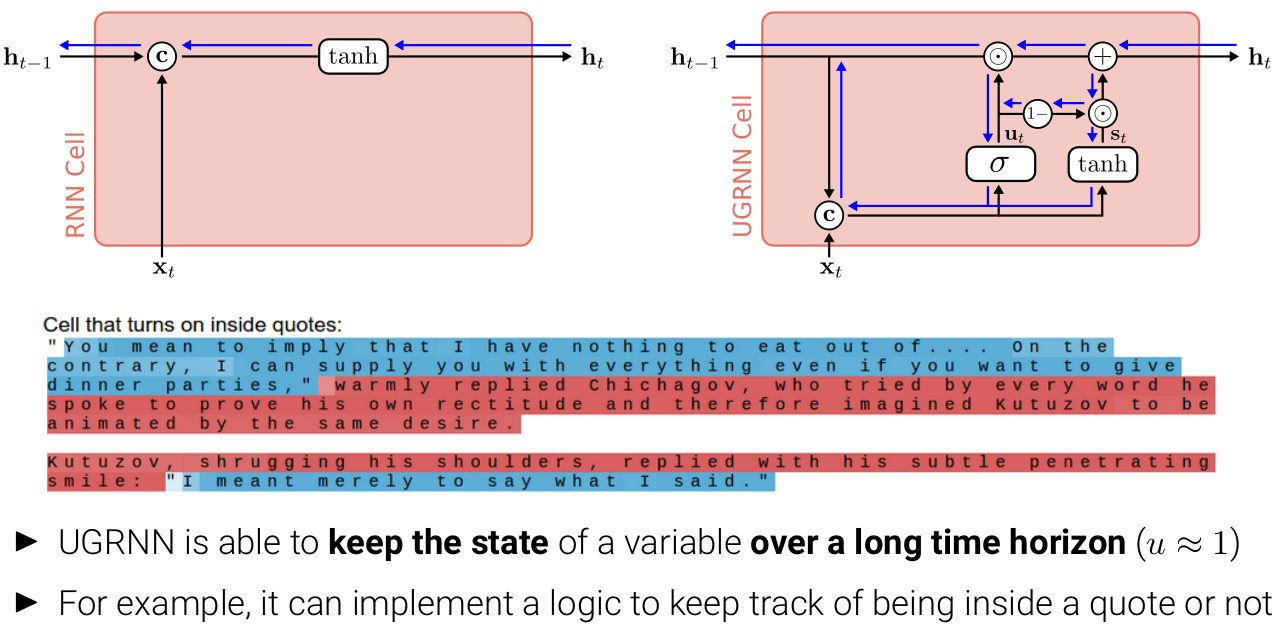
\includegraphics[width=.95\textwidth]{images/s19}
\end{center}
\end{frame}

\begin{frame}
  \frametitle{Gated Recurrent Unit (GRU)}
\begin{center}
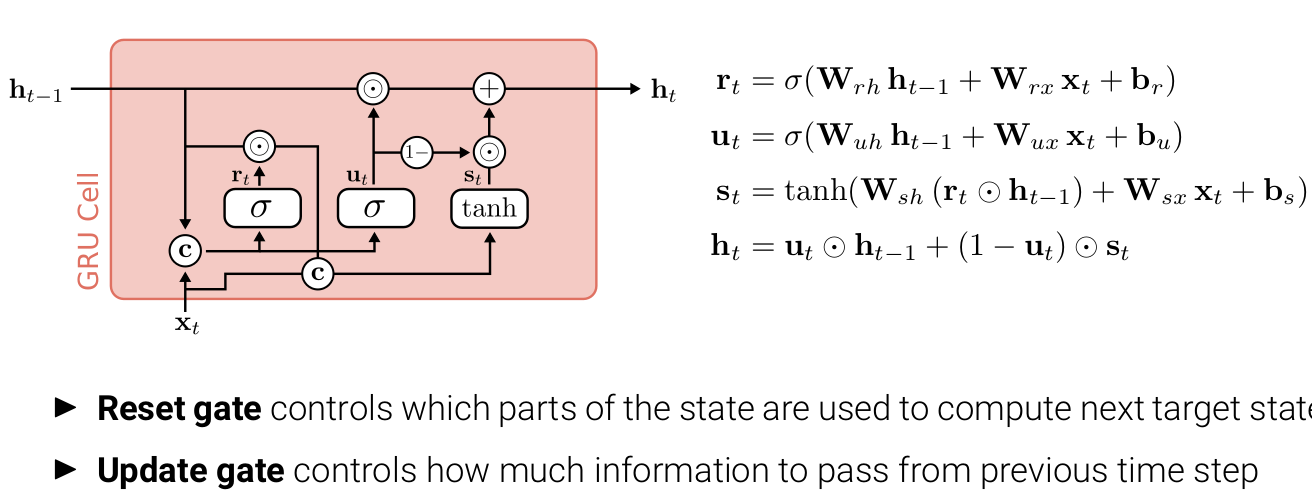
\includegraphics[width=.9\textwidth]{images/s20}
\end{center}
\end{frame}

\begin{frame}
  \frametitle{Gated Recurrent Unit (GRU)}
\begin{center}
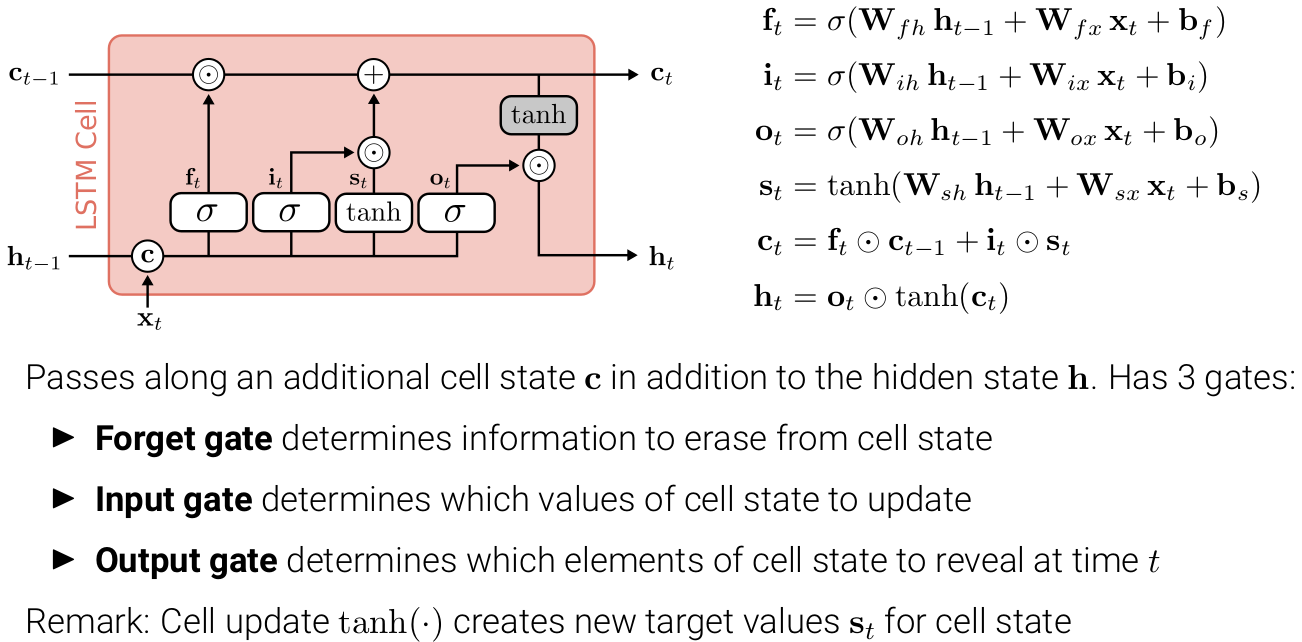
\includegraphics[width=.95\textwidth]{images/s21}
\end{center}
\end{frame}

\begin{frame}
  \frametitle{Gated Recurrent Unit (GRU)}
\begin{center}
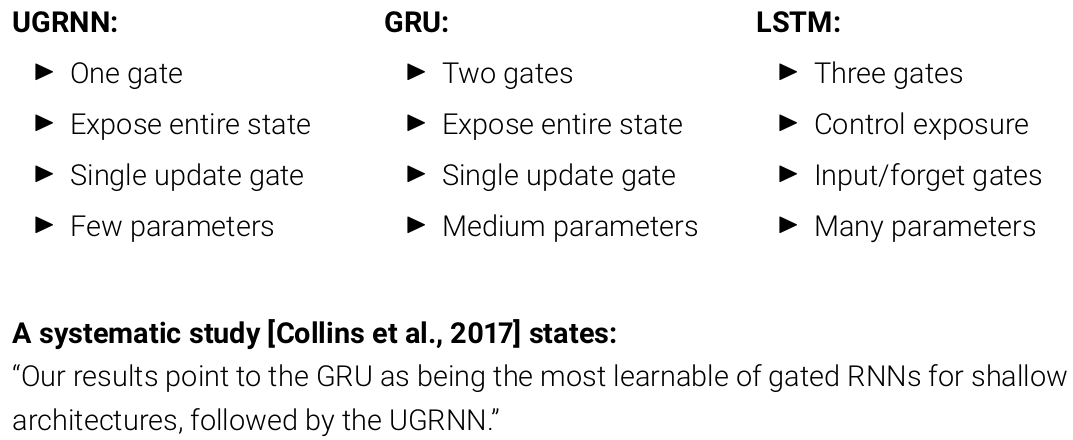
\includegraphics[width=.95\textwidth]{images/missing}
\end{center}
\end{frame}


\begin{frame}
  \frametitle{Sequence to Sequence Learning}
\begin{center}
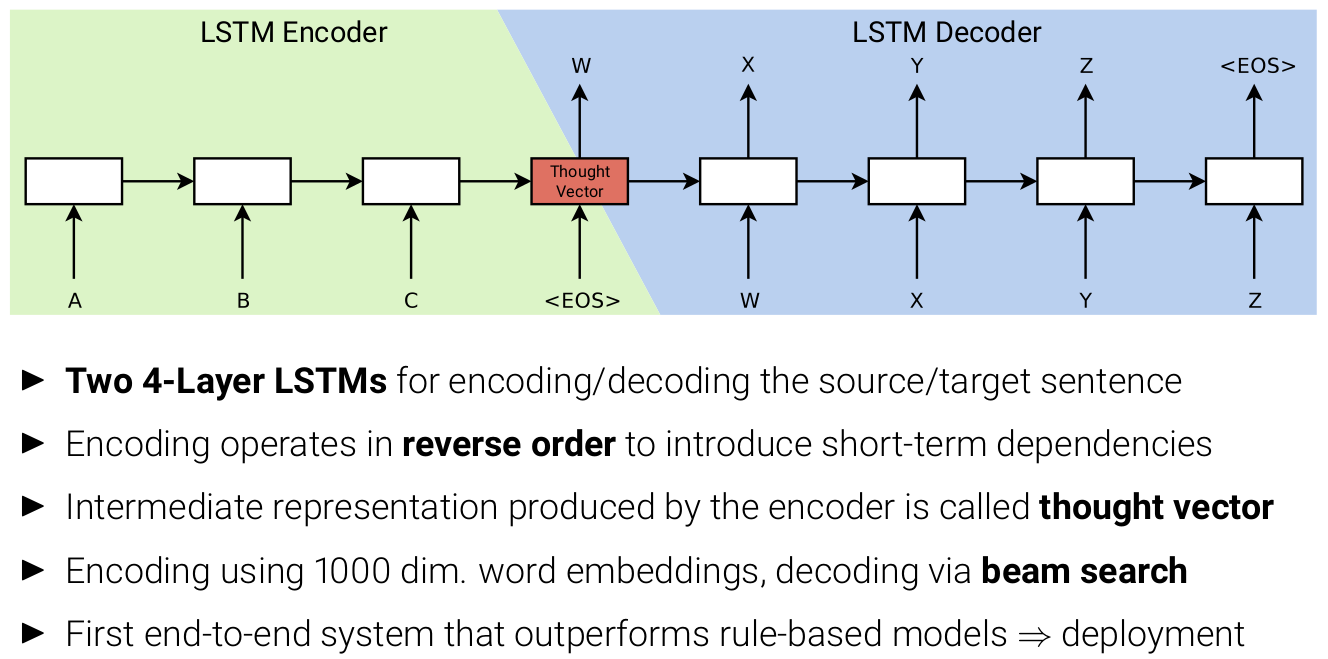
\includegraphics[width=.9\textwidth]{images/sa}
\end{center}
\scriptsize{Sutskever, Vinyals and Le: Sequence to Sequence Learning with Neural Networks. NIPS, 2014}
\end{frame}


\begin{frame}
  \frametitle{Decoding}
\begin{center}
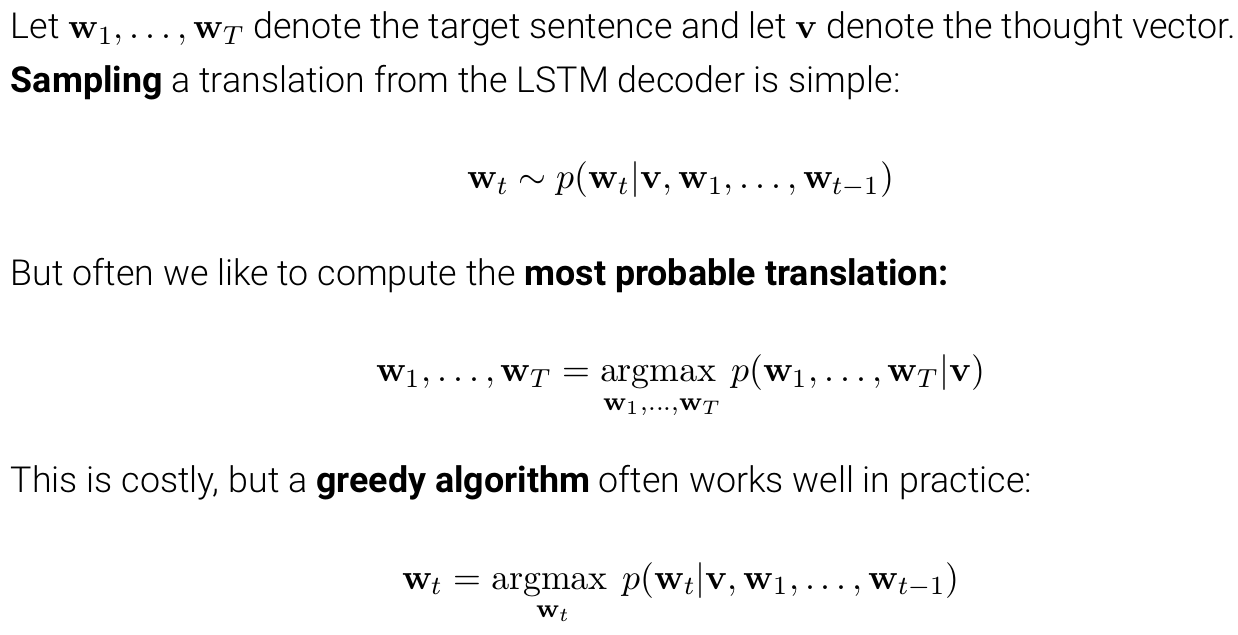
\includegraphics[width=.85\textwidth]{images/sb}
\end{center}
\scriptsize{Sutskever, Vinyals and Le: Sequence to Sequence Learning with Neural Networks. NIPS, 2014}
\end{frame}


\begin{frame}
  \frametitle{Beam Search}
\begin{center}
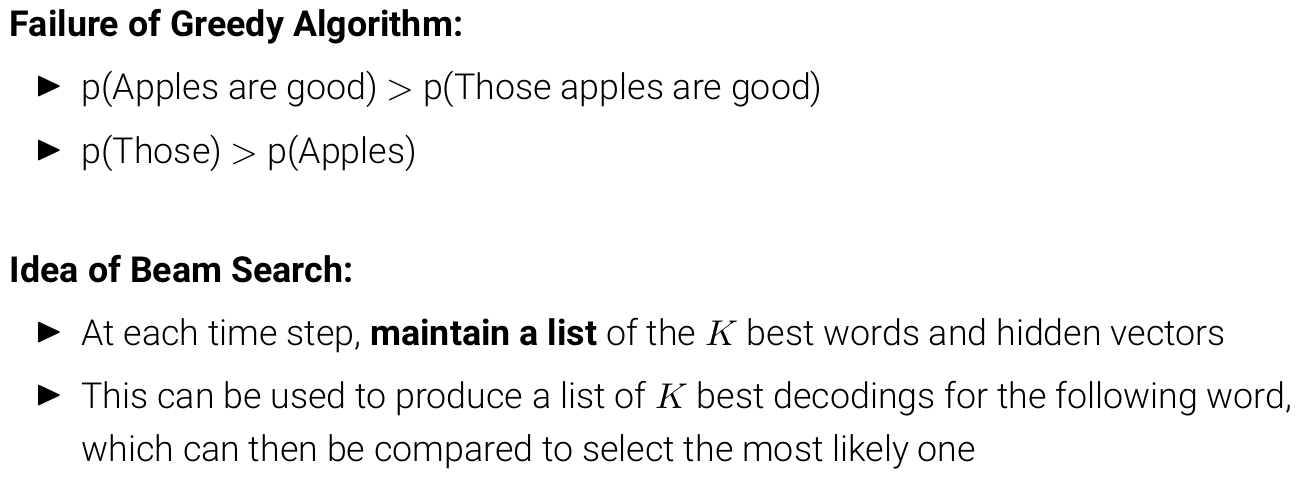
\includegraphics[width=.95\textwidth]{images/sc}
\end{center}
\scriptsize{Sutskever, Vinyals and Le: Sequence to Sequence Learning with Neural Networks. NIPS, 2014}
\end{frame}

\begin{frame}
  \frametitle{Beam Search}
\begin{center}
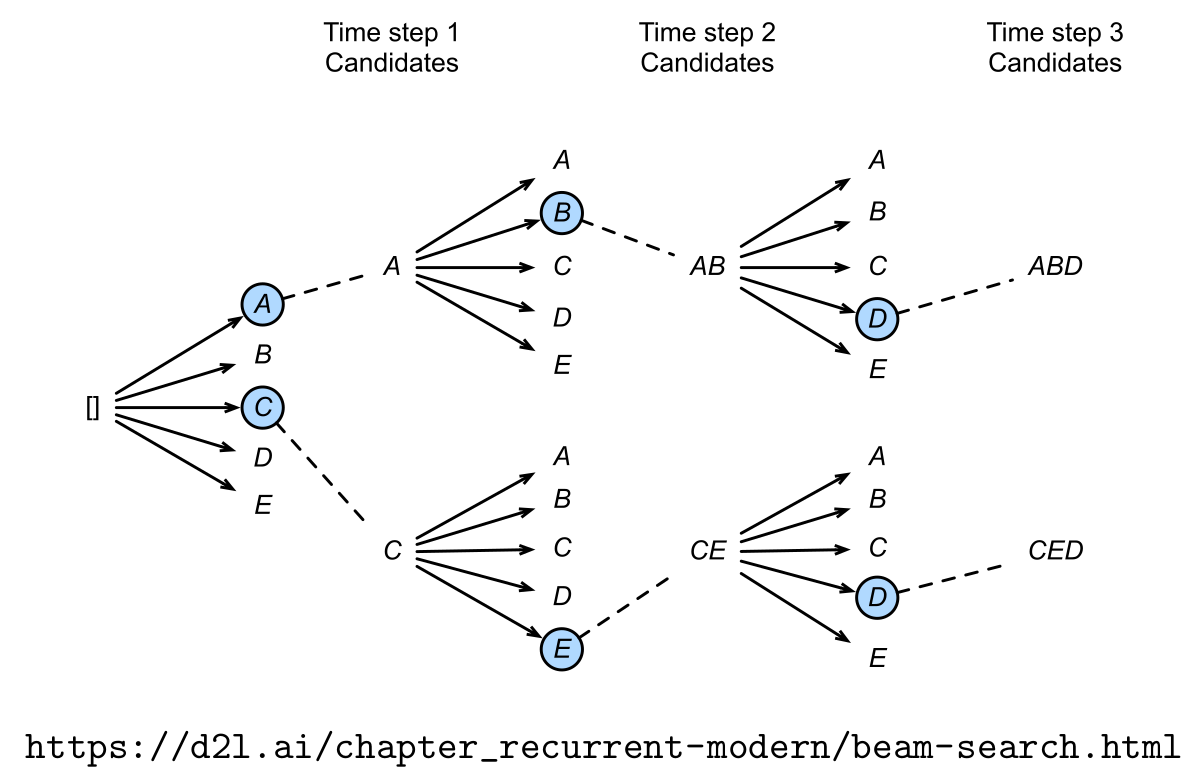
\includegraphics[width=.7\textwidth]{images/sd}
\end{center}
\scriptsize{Sutskever, Vinyals and Le: Sequence to Sequence Learning with Neural Networks. NIPS, 2014}
\end{frame}


\section{Attention and Transformers} 

\begin{frame}
  \frametitle{Attention}
\begin{center}
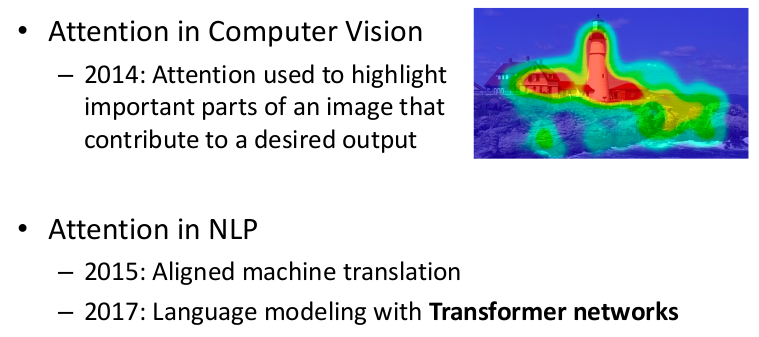
\includegraphics[width=.9\textwidth]{images/p1}
\end{center}

\scriptsize{Vaswani, Shazeer, Parmar, Uszkoreit, Jones, Gomez, Kaiser and Polosukhin: Attention is All you Need. NIPS, 2017.}
\end{frame}


\begin{frame}
  \frametitle{Attention}
\begin{center}
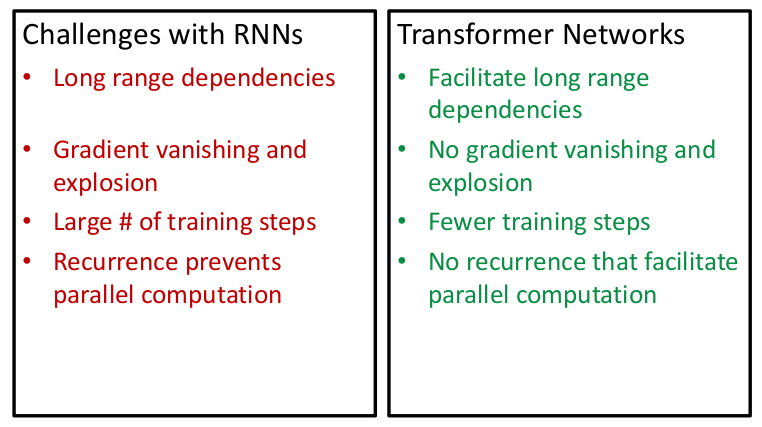
\includegraphics[width=.8\textwidth]{images/p2}
\end{center}
\end{frame}

\begin{frame}
  \frametitle{Attention Mechanism}
 
\begin{itemize}[<+->]
\item Mimics the retrieval of a \textbf{value} $v_i$ for a \textbf{query} $q$
based on a \textbf{key} $k_i$ in a database
\item In a probabilistic way
\begin{align*}
\text{attention}(q,\textbf{k},\textbf{v}) & = \sum_i \underbrace{\text{similarity}(q,k_i)}_{\alpha_i}\cdot v_i
\end{align*}
\item The \textbf{query} $q$ and \textbf{key} $k_i$ are embedding vectors
\item Typically, $\text{similarity}$ is chosen to be the dot product
\item The produced output is a linear combination of values (also embedding vectors) $v_i$
\item Example:
\begin{itemize}
\item $q$ : possible question (Q)
\item $k_i$ : potentially useful information to answer (K)
\item $v_i$ : potential answer (V)
\end{itemize}
\item Everything is learned from data
\end{itemize}
\end{frame}

\begin{frame}
  \frametitle{The Transformer Network}
  \begin{columns}
    \column[c]{.55\textwidth}    
\begin{itemize}
\setlength\itemsep{.8em}
\item Initially developed for machine translation
\item No recurrence
\begin{itemize}
\item Input: entire sequence to translate
\item Output: entire translated sequence
\end{itemize}
\item Encoder-decoder based on attention 
\item Key idea: learns abstract embeddings
\begin{itemize}
\item 1st layer: pairs of embeddings
\item 2st layer: pairs of pairs of embeddings
\item Up to $N=6$ layers
\end{itemize}
\end{itemize}
    \column[c]{.45\textwidth}
\begin{center}
	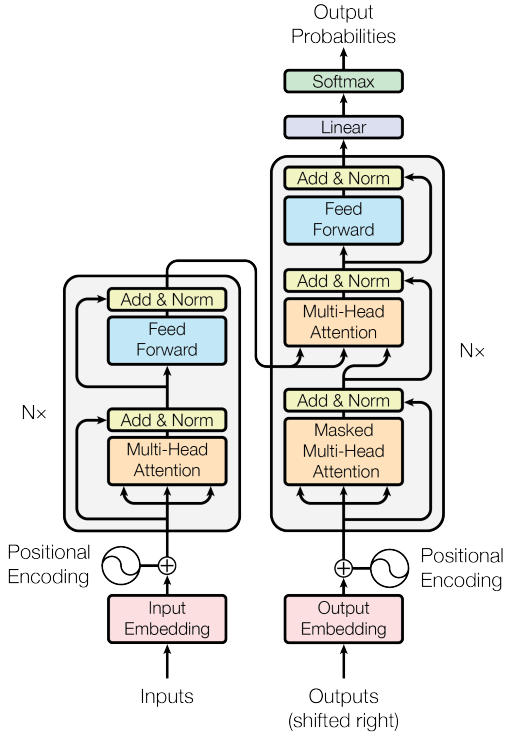
\includegraphics[width=.7\columnwidth]{images/transf}
\end{center}
    \end{columns}
\scriptsize{Vaswani, Shazeer, Parmar, Uszkoreit, Jones, Gomez, Kaiser and Polosukhin: Attention is All you Need. NIPS, 2017.}
\end{frame}


\begin{frame}
  \frametitle{The Transformer Network: Encoder}
  \begin{columns}
    \column[c]{.7\textwidth}    
\begin{itemize}
\setlength\itemsep{.8em}
\item Input embedding: zero-order embedding (size $n$)
\item Positional Encodings: concatenates positional information
\item Multi-headed attention (see next slide)
\item Normalization layer: reduces "covariance shift" and speeds up converge
\item Feedforward layer: shared weights within layer 
\item Output: a higher order embedding of the sentence (size $n$)
\end{itemize}
    \column[c]{.3\textwidth}
\begin{center}
	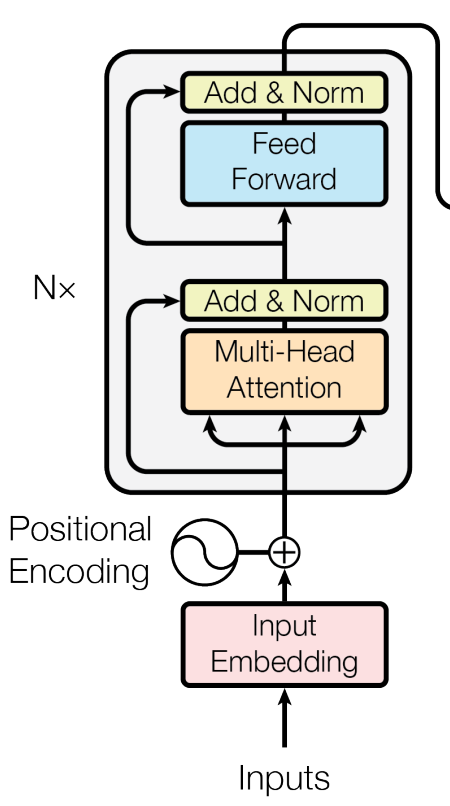
\includegraphics[width=.6\columnwidth]{images/enc}
\end{center}
    \end{columns}
\vspace{.75cm}
\scriptsize{Vaswani, Shazeer, Parmar, Uszkoreit, Jones, Gomez, Kaiser and Polosukhin: Attention is All you Need. NIPS, 2017.}
\end{frame}


\begin{frame}
  \frametitle{Attention in the Transformer}

  \begin{columns}
    \column[c]{.47\textwidth}    
\begin{center}
	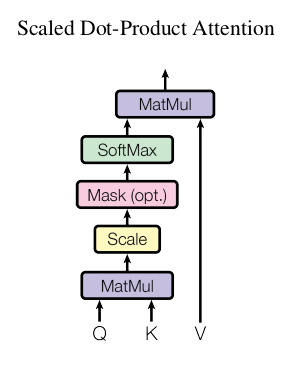
\includegraphics[width=.55\columnwidth]{images/att1}
\end{center}
    \column[c]{.52\textwidth}
\begin{center}
	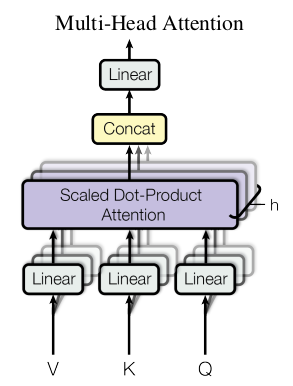
\includegraphics[width=.47\columnwidth]{images/att2}
\end{center}
    \end{columns}
\begin{itemize}
\item Three types of attention modules
\begin{itemize}
\item Encoder: self-attention (key, value and query are input embeddings) 
\item Encoder $\rightarrow$ Decoder : query (output embedding), key and value (input embeddings) 
\item Decoder: self-attention (key, value and query are input embeddings)
and masked attention (prevents attending future words)
\end{itemize}
\end{itemize}

\end{frame}


\begin{frame}
  \frametitle{Attention in the Transformer}

  \begin{columns}
    \column[c]{.47\textwidth}    
\begin{center}
	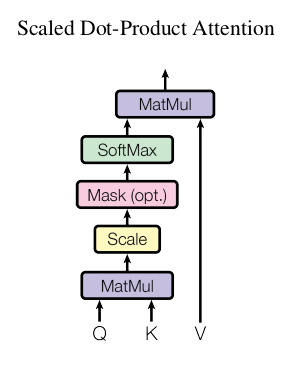
\includegraphics[width=.55\columnwidth]{images/att1}
\end{center}
    \column[c]{.52\textwidth}
\begin{center}
	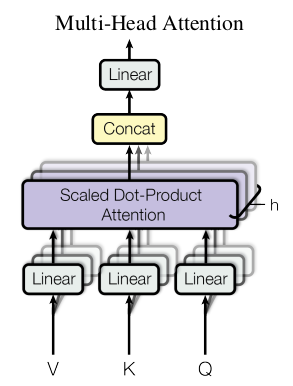
\includegraphics[width=.47\columnwidth]{images/att2}
\end{center}
    \end{columns}
\begin{itemize}
\item Multi-head attention
\begin{itemize}
\item Computer multiple attentions per query with different weights
\item Lets network learn different semantic meanings of attention
\end{itemize}
\end{itemize}
\end{frame}

\begin{frame}
  \frametitle{Multi-headed Attention Visualization}
\begin{center}
	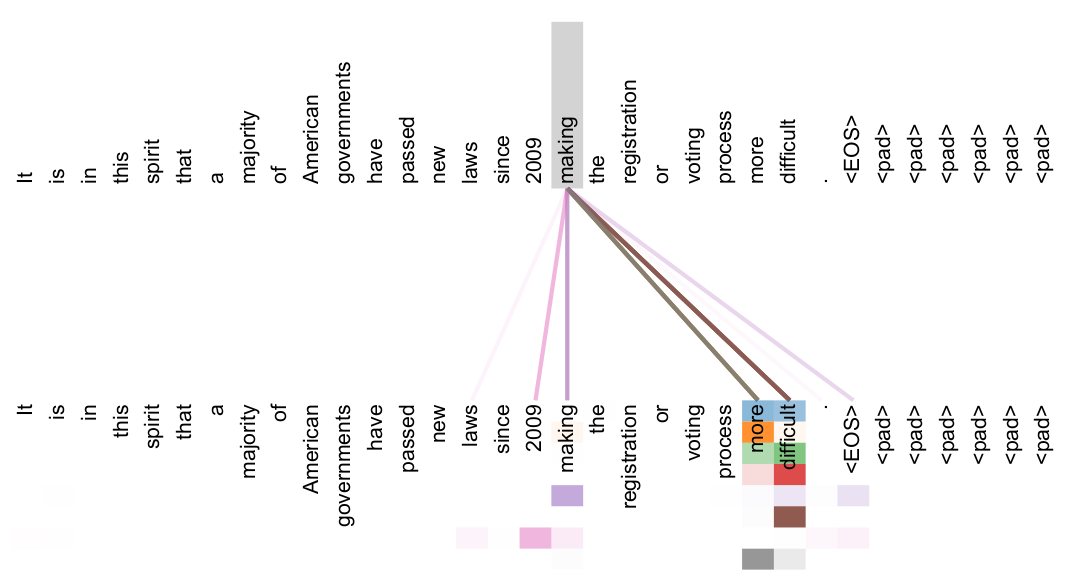
\includegraphics[width=.9\columnwidth]{images/attnA}
\end{center}
\end{frame}


\begin{frame}
  \frametitle{The Transformer Network: Decoder}
  \begin{columns}
    \column[c]{.7\textwidth}    
\begin{itemize}
\setlength\itemsep{.8em}
\item Similar to encoder
\item When decoding, an output value should only depend on previous outputs
\item Masked multi-head attention: multi-head where some values are 
masked (i.e., probabilisties of masked values are nullified to prevent them from being selected)
\item Teacher forcing (trained with correct output word)
\end{itemize}
    \column[c]{.3\textwidth}
\begin{center}
	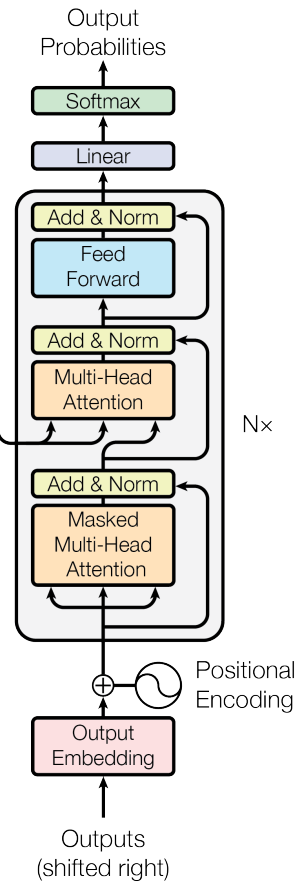
\includegraphics[width=.5\columnwidth]{images/dec}
\end{center}
    \end{columns}
\vspace{.25cm}
\scriptsize{Vaswani, Shazeer, Parmar, Uszkoreit, Jones, Gomez, Kaiser and Polosukhin: Attention is All you Need. NIPS, 2017.}
\end{frame}

\begin{frame}
  \frametitle{Transformer-based Models (BERT)}
{\color{red}\textbf{BERT}: Pre-training of Deep Bidirectional Transformers for Language Understanding}

\begin{itemize}
\setlength\itemsep{.8em}
\item Does not predict next words sequentially
\item Uses a context composed of previous and future words
\item Masked language modeling (MLM) like ``fill the gaps''
\item Text encoding, summarization, Question Answering
\item Two training phases
\begin{itemize}
\item First: unsupervised training (basically a Transformer \textbf{Encoder} stack)
\item Second: specific fine-tuning for a particular task
\end{itemize} 
\end{itemize} 
\vspace{.5cm}
\scriptsize{Devlin et al. BERT: Pre-training of Deep Bidirectional Transformers for Language Understanding (2018)}
\end{frame}

\begin{frame}
  \frametitle{Transformer-based Models (GPT)}
{\color{red}Generative Pretrained Transformer (\textbf{GPT-x})}

\begin{itemize}
\setlength\itemsep{.3em}
\item Basically a Transformer \textbf{Decoder} stack
\item Trained unsupervised on a large corpus to predict the next word
\item ``prompts'' the language model with different inputs
\end{itemize}
	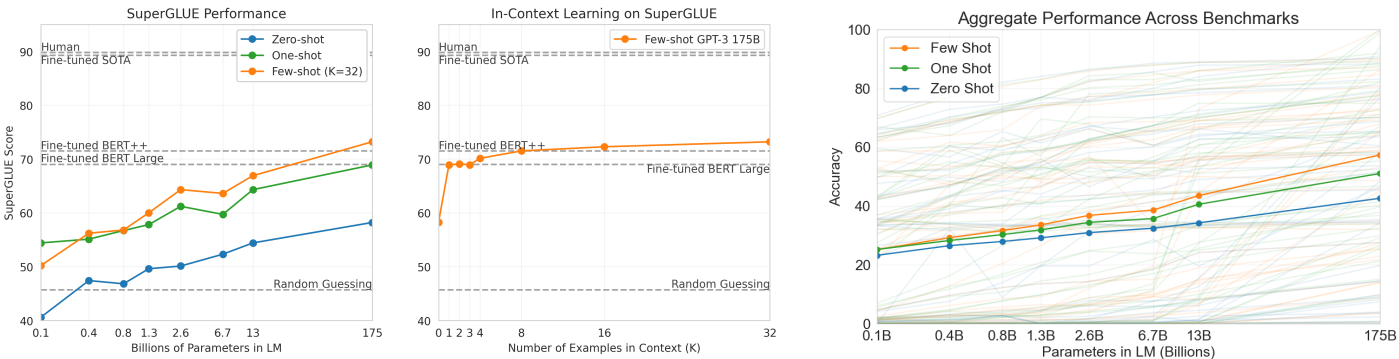
\includegraphics[width=\columnwidth]{images/gptc}
\vspace{.05cm}

\scriptsize{Radford et al. Language models are unsupervised multitask learners (2019).\\
Brown et al. Language Models are Few-Shot Learners (2020)}
\end{frame}

\begin{frame}
  \frametitle{Transformer-based Models (GPT)}
{\color{red}Generative Pretrained Transformer (\textbf{GPT-x})}
\begin{itemize}
\item GPT-2 sizes
\end{itemize}
\begin{center}
	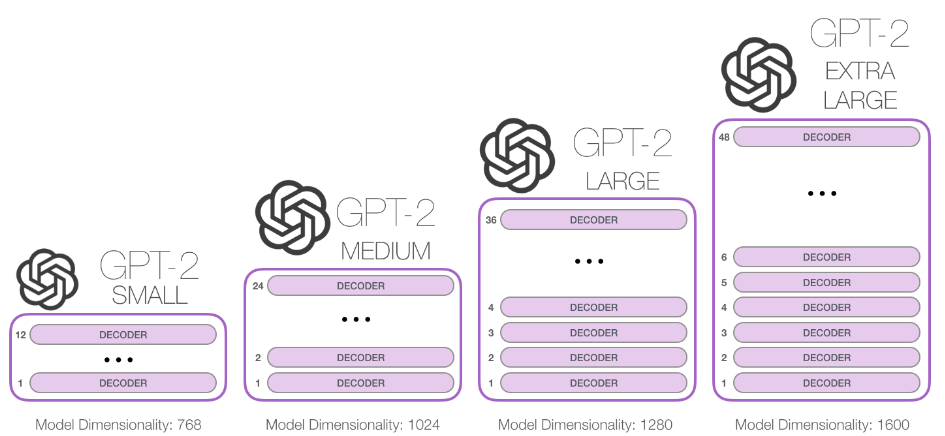
\includegraphics[width=.7\columnwidth]{images/gpt2}
\end{center}
\vspace{.05cm}

\scriptsize{Radford et al. Language models are unsupervised multitask learners (2019).\\
Brown et al. Language Models are Few-Shot Learners (2020)}
\end{frame}


\begin{frame}
  \frametitle{Examples of fine-tuning (GPT)}
{\color{red}Generative Pretrained Transformer (\textbf{GPT-x})}
\begin{itemize}[<+->]
\item {\color{blue}{Task:}} Given some text, generate a natural continuation with \textbf{positive} sentiment:
(fine-tuning GPT2 with 5000 human samples suffice for strong performance according to humans)
\item \textbf{Context (input):} \texttt{She looked tired. She’d been crying.
Next to her was a man of medium build and unremarkable height, with brown hair just tousled enough to be fashionable. He wore a grey suit, its gravity somewhat offset by a black tie that featured Marvin the Martian. I recognized him.}
\item \textbf{Zero-shot baseline:}
\texttt{He was the guy who’d been chasing me the day I’d arrived in the city.}
\item \textbf{fine-tuning:}
\texttt{He smiled at me and I smiled back. He was pleasant enough, for a man of his age.}
\end{itemize}
\end{frame}


\begin{frame}
  \frametitle{Examples of fine-tuning (GPT)}
{\color{red}Generative Pretrained Transformer (\textbf{GPT-x})}
\begin{itemize}[<+->]
\item {\color{blue}{Task:}} Given some text, generate a natural continuation with \textbf{physically descriptive text}:
(fine-tuning GPT2 with 5000 human samples suffice for strong performance according to humans)
\item \textbf{Context (input):} \texttt{It’s not her fault I was in a bad mood today. Not her fault I stayed up all night then took it out on her.
In a way, she’s like basketball for me. An escape.
Maybe a much moodier escape, but one all the same.}
\item \textbf{Zero-shot baseline:}
\texttt{I’m standing in the kitchen, trying to decide if I should call her when she comes bustling in.}
\item \textbf{fine-tuning:}
\texttt{
I pause on the steps, listening to the distant sound of music playing from the living room.
looked tired. She’d been crying.}
\end{itemize}
\end{frame}


\begin{frame}
  \frametitle{Transformer-based Models (GPT)}
\begin{itemize}
\item Examples of few-shot learning
\end{itemize}
\begin{center}
	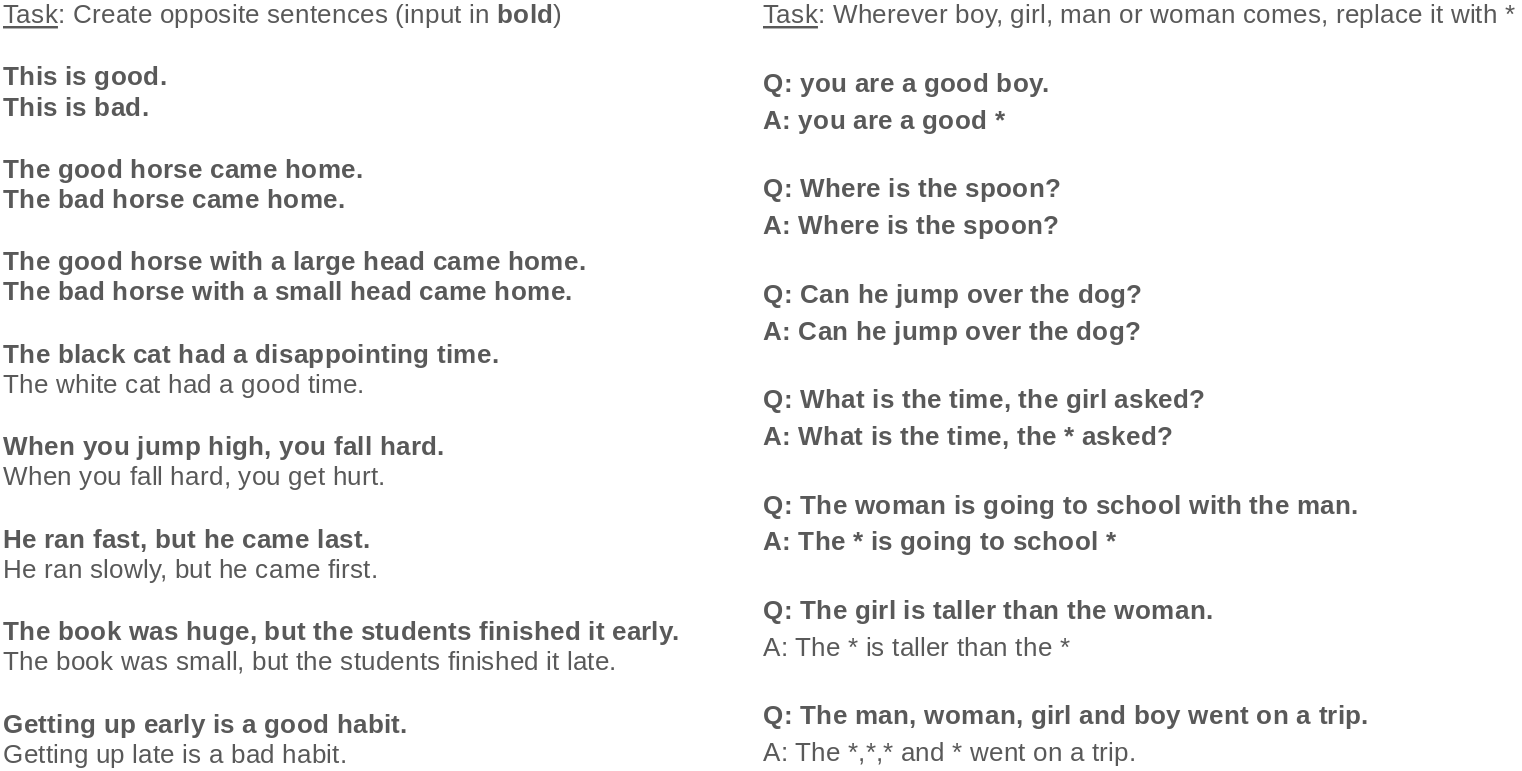
\includegraphics[width=.9\columnwidth]{images/zeroshot}
\end{center}
\end{frame}




\begin{frame}
  \frametitle{Problems and Controversy}
Far from \textbf{understanding} languange
\begin{center}
	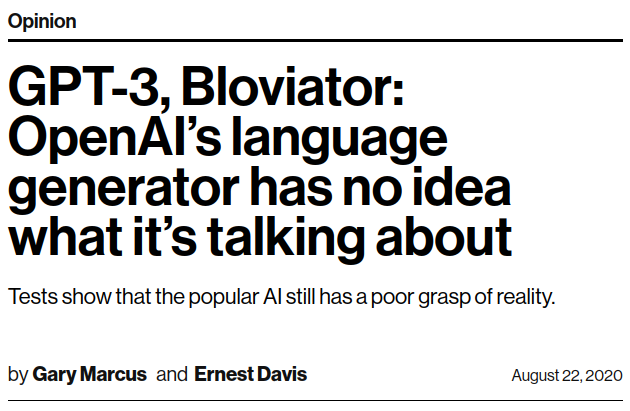
\includegraphics[width=.5\columnwidth]{images/pr1}
\end{center}
\vspace{.25cm}
\scriptsize{
\url{https://www.technologyreview.com/2020/08/22/1007539/gpt3-openai-language-generator-artificial-intelligence-ai-opinion/
}}
\end{frame}





\begin{frame}
  \frametitle{Problems and Controversy}
\begin{center}
	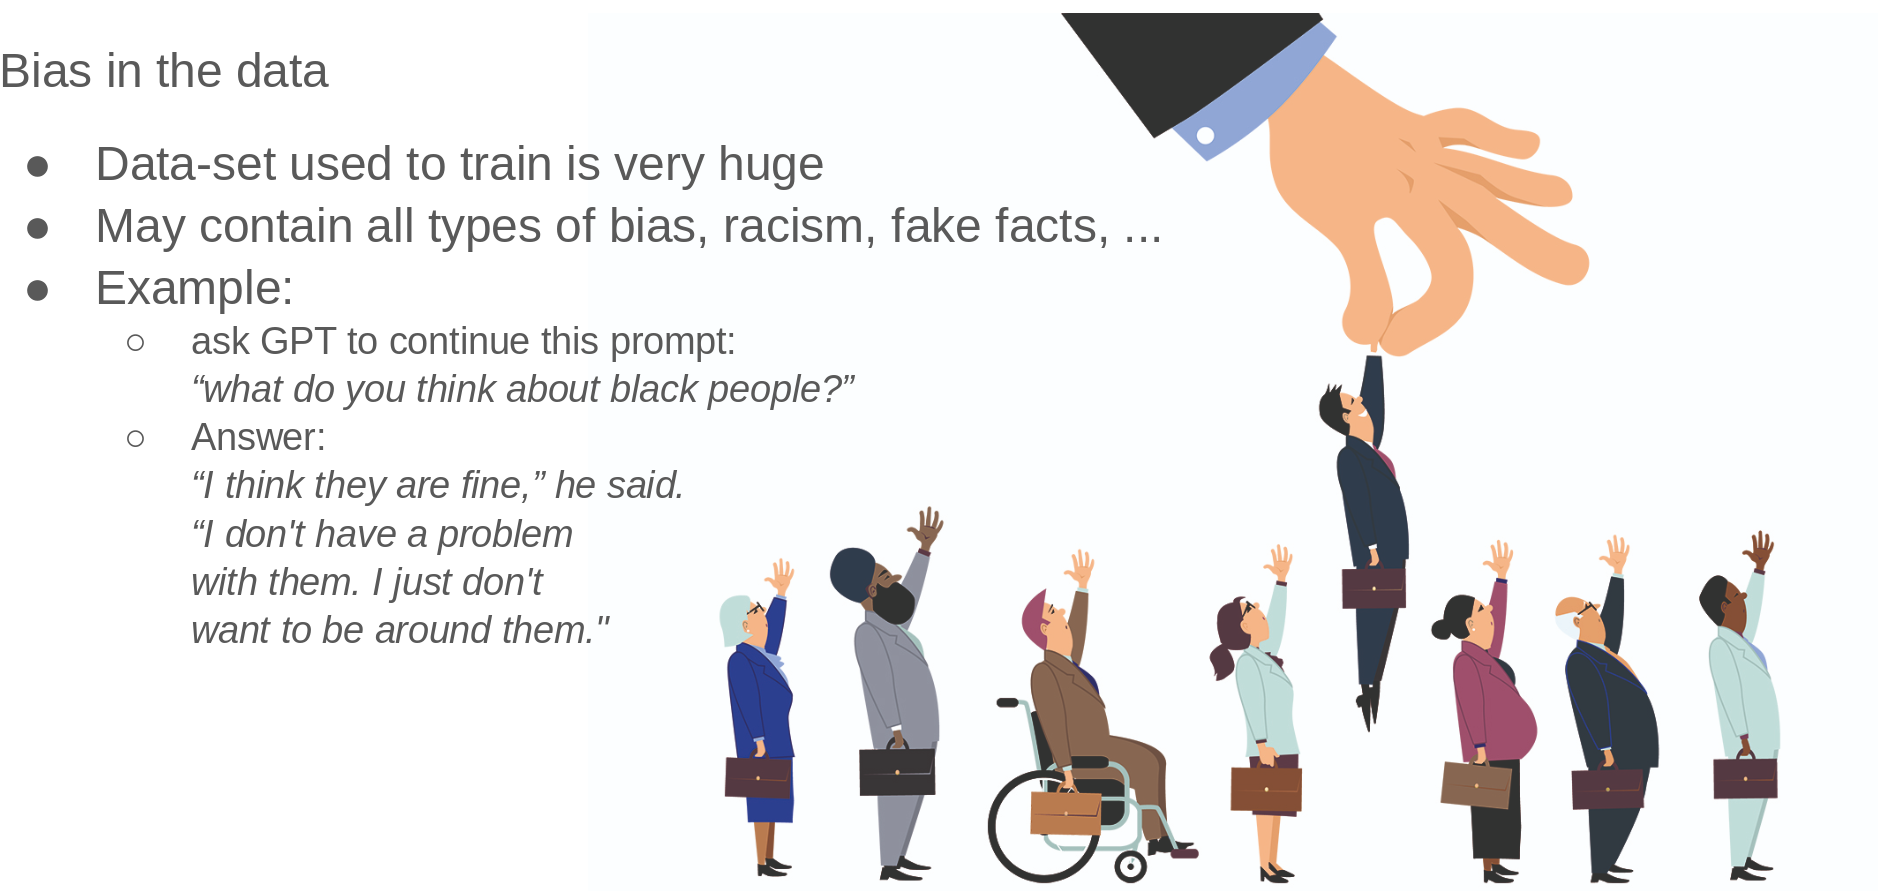
\includegraphics[width=\columnwidth]{images/pr2}
\end{center}
\end{frame}

\begin{frame}
  \frametitle{Problems and Controversy}
\begin{center}
	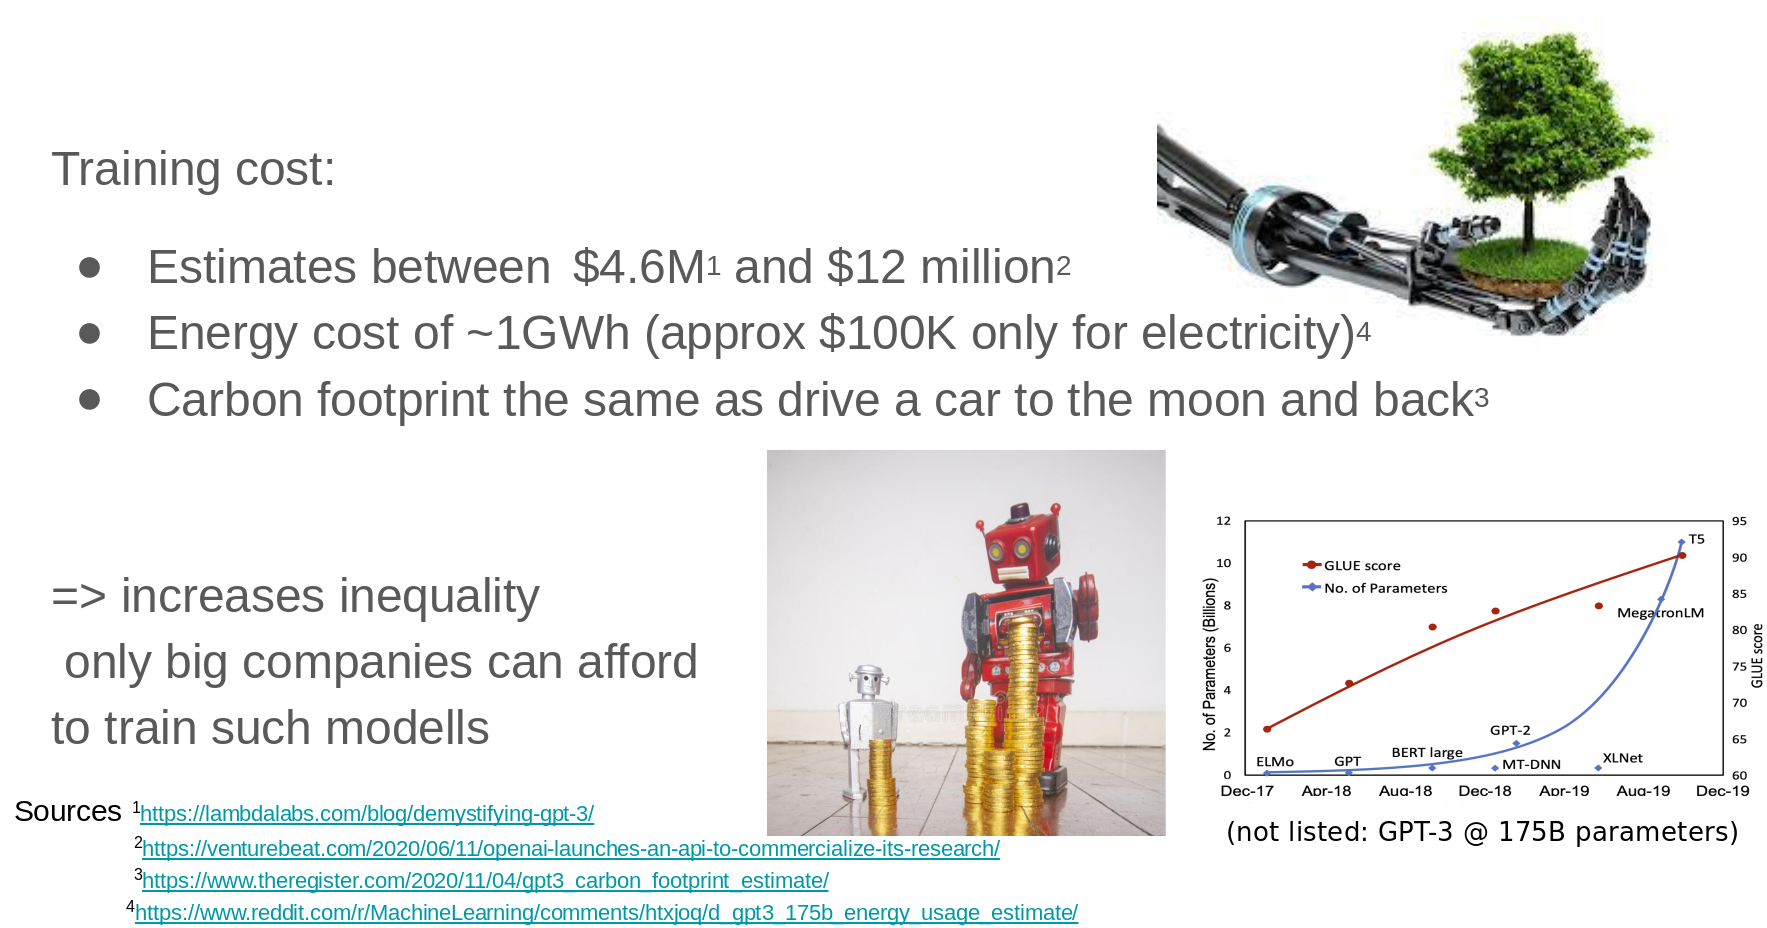
\includegraphics[width=\columnwidth]{images/pr3}
\end{center}
\end{frame}


\begin{frame}
  \frametitle{Problems and Controversy}
\begin{center}
	
\includegraphics[width=\columnwidth]{images/pr4}
\end{center}
\end{frame}


\begin{frame}
  \frametitle{Resources}

\begin{itemize}
\setlength\itemsep{1em}
\item Deep Learning (Lectures 8,9) Prof. Andreas Geiger, University of T\"ubingen
{\scriptsize{\url{https://uni-tuebingen.de/fakultaeten/mathematisch-naturwissenschaftliche-fakultaet/fachbereiche/informatik/lehrstuehle/autonomous-vision/lectures/deep-learning/}}}
\item CS480/680 Lecture 19: Attention and Transformer Networks
{\scriptsize{\url{https://www.youtube.com/watch?v=OyFJWRnt_AY&list=PLVBRFV4GMJLxRYlPVWcWFvEyXsdQbl_1J&index=14&ab_channel=PascalPoupart}}}
\end{itemize}
\end{frame}





%\begin{frame}
%  \frametitle{The transformer}
%\begin{itemize}[<+->]
%\setlength\itemsep{.8em}
%\item \textbf{Attention based} model which does not rely on recurrence nor convolutions
%\item Process all tokens in \textbf{parallel} (not sequentially as in an RNN)
%\item Leads to significant speed-ups when using modern GPU clusters
%\item \textbf{Self-attention} relates all tokens in a layer with each other
%\item Thus can more easily capture \textbf{long-distance dependencies} compared to RNNs
%\item Transformer-like architectures have now replaced RNNs in NLP applications,
%\textbf{Defacto standard} for all state-of-the-art models
%\end{itemize}
%\vspace{1cm}
%\scriptsize{Vaswani, Shazeer, Parmar, Uszkoreit, Jones, Gomez, Kaiser and Polosukhin: Attention is All you Need. NIPS, 2017.}
%\end{frame}

%\begin{frame}
%  \frametitle{BERT (Bidirectional Encoder Representations from Transformers)}
%Full architecture
%\end{frame}



%\begin{frame}
%  \frametitle{Recurrent Neural Networks}
%\begin{itemize}
%\item Deal with inputs as sequences of variable lengths
%\item Simplest architecture
%\end{itemize}
%\begin{center}
%\includegraphics[width=.3\textwidth]{images/rnn1}
%\end{center}
%\begin{align*}
%W
%\end{align*}
%\end{frame}


\section{Application: Language Models}



\end{document}
